%%%%%%%%%%%%%%%%%%%%%%%%%%%%%%% beamer %%%%%%%%%%%%%%%%%%%%%%%%%%%%%%%%%%%%%%%%%%%%%%%%%
% To run - pdflatex filename.tex
%      acroread filename.pdf
%%%%%%%%%%%%%%%%%%%%%%%%%%%%%%%%%%%%%%%%%%%%%%%%%%%%%%%%%%%%%%%%%%%%%%%%%%%%%%%%%%%%%%%%

\documentclass[compress,oilve]{beamer}
\mode<presentation>

\usetheme[]{CambridgeUS}
% other themes: AnnArbor, Antibes, Bergen, Berkeley, Berlin, Boadilla, boxes, CambridgeUS, Copenhagen, Darmstadt, default, Dresden, Frankfurt, Goettingen,
% Hannover, Ilmenau, JuanLesPins, Luebeck, Madrid, Maloe, Marburg, Montpellier, PaloAlto, Pittsburg, Rochester, Singapore, Szeged, classic

\usecolortheme{beaver}
% color themes: albatross, beaver, beetle, crane, default, dolphin,  fly, lily, orchid, rose, seagull, seahorse, sidebartab, whale, wolverine

\usefonttheme{professionalfonts}
% font themes: default, professionalfonts, serif, structurebold, structureitalicserif, structuresmallcapsserif


\hypersetup{pdfpagemode=FullScreen} % makes your presentation go automatically to full screen

% define your own colors:
\definecolor{Red}{rgb}{1,0,0}
\definecolor{Blue}{rgb}{0,0,1}
\definecolor{Green}{rgb}{0,1,0}
\definecolor{magenta}{rgb}{1,0,.6}
\definecolor{lightblue}{rgb}{0,.5,1}
\definecolor{lightpurple}{rgb}{0.8, 0.6, 0.9}
\definecolor{gold}{rgb}{.6,.5,0}
\definecolor{orange}{rgb}{1,0.4,0}
\definecolor{hotpink}{rgb}{1,0,0.5}
\definecolor{newcolor2}{rgb}{.5,.3,.5}
\definecolor{newcolor}{rgb}{0,.3,1}
\definecolor{newcolor3}{rgb}{1,0,.35}
\definecolor{darkgreen1}{rgb}{0, .35, 0}
\definecolor{darkgreen}{rgb}{0, .6, 0}
\definecolor{darkred}{rgb}{.75,0,0}
\definecolor{skyblue}{HTML}{75bbfd}

\definecolor{olive}{cmyk}{0.64,0,0.95,0.4}
\definecolor{purpleish}{cmyk}{0.75,0.75,0,0}

% can also choose different themes for the "inside" and "outside"

% \usepackage{beamerinnertheme_______}
% inner themes include circles, default, inmargin, rectangles, rounded

% \usepackage{beamerouterthemesmoothbars}
% outer themes include default, infolines, miniframes, shadow, sidebar, smoothbars, smoothtree, split, tree


\useoutertheme[subsection=true, height=40pt]{smoothbars}

% to have the same footer on all slides
%\setbeamertemplate{footline}[text line]{STUFF HERE!}
\setbeamertemplate{footline}[text line]{} % makes the footer EMPTY
% include packages
%

%show the page numbers in footnote
%\addtobeamertemplate{navigation symbols}{}{%
%	\usebeamerfont{footline}%
%	\usebeamercolor[fg]{footline}%
%	\hspace{1em}%
%	\insertframenumber/\inserttotalframenumber
%}

\setbeamercolor{footline}{fg=purpleish}
\setbeamerfont{footline}{series=\bfseries}

%add color to curent subsection
\setbeamertemplate{section in head/foot}{\hfill\tikz\node[rectangle, fill=darkred, rounded corners=1pt,inner sep=1pt,] {\textcolor{white}{\insertsectionhead}};}
\setbeamertemplate{section in head/foot shaded}{\textcolor{darkred}{\hfill\insertsectionhead}}

% Remove bullet of subsections
\setbeamertemplate{headline}
{%
	\begin{beamercolorbox}{section in head/foot}
		\insertsectionnavigationhorizontal{\textwidth}{}{}
	\end{beamercolorbox}%
}


% modify headlline, specially headline size
\setbeamertemplate{headline}{%
	\leavevmode%
	\hbox{%
		\begin{beamercolorbox}[wd=\paperwidth,ht=3.5ex,dp=1.125ex]{palette quaternary}%
			\insertsectionnavigationhorizontal{\paperwidth}{}{\hskip0pt plus1filll}
		\end{beamercolorbox}%
	}
}

\setbeamertemplate{footline}{%
	\leavevmode%
	\hbox{\begin{beamercolorbox}[wd=.5\paperwidth,ht=2.5ex,dp=1.125ex,leftskip=.3cm plus1fill,rightskip=.3cm]{author in head/foot}%
			\usebeamerfont{author in head/foot}\insertshortauthor ~ \insertshortinstitute
		\end{beamercolorbox}%
		\begin{beamercolorbox}[wd=.5\paperwidth,ht=2.5ex,dp=1.125ex,leftskip=.3cm,rightskip=.3cm plus1fil]{title in head/foot}%
			\usebeamerfont{title in head/foot}\insertshorttitle\hfill\insertframenumber\,/\,\inserttotalframenumber
	\end{beamercolorbox}}%
	\vskip0pt%
}


%\setbeamertemplate{navigation symbols}{}

\title{Recurrent Networks}
\author{ML Instruction Team, Fall 2022}
\institute[]{CE Department \newline  Sharif University of Technology \newline \newline}
\date[\today]{}
%\titlegraphic{\includegraphics[scale=.35]{example-image}}



%Write \usepackage{etex} just after the \documentclass line (it should be the first loaded package).
\usepackage{etex}
\usepackage{subcaption}
\usepackage{multicol}
\usepackage{amsmath}
\usepackage{epsfig}
\usepackage{graphicx}
\usepackage[all,knot]{xy}
\xyoption{arc}
\usepackage{url}
\usepackage{multimedia}
\usepackage{hyperref}
\hypersetup{colorlinks,linkcolor=blue,citecolor=redorange,urlcolor=darkred}
\usepackage{multirow}
\usepackage[font={scriptsize}]{caption}
\usepackage{pgf}
\usepackage{fontspec}
%\setsansfont[Scale=MatchLowercase, BoldFont = * Bold, ItalicFont = * Italic]{Caladea}

%\usepackage{enumitem,xcolor}
%\newcommand{\labelitemi}{$\blacksquare$}
%\newcommand{\labelitemii}{$\diamond$}
%\newcommand{\labelitemiii}{$\square$}
%\newcommand{\labelitemiv}{$\ast$}
%\setbeamercolor*{item}{fg=red}


\usefonttheme{professionalfonts} 
\setbeamertemplate{itemize item}{\color{skyblue}$\blacksquare$}
\setbeamertemplate{itemize subitem}{\color{hotpink}$\blacktriangleright$}
\setbeamertemplate{itemize subsubitem}{\color{orange}$\bullet$}


\usepackage{anyfontsize}
\usepackage{t1enc}
\usepackage{tikz}
\usetikzlibrary{calc,trees,positioning,arrows,chains,shapes.geometric,decorations.pathreplacing,decorations.pathmorphing,shapes,matrix,shapes.symbols}



\newtheorem{proposition}[theorem]{Proposition}
\newtheorem{remark}[theorem]{Remark}
\newtheorem{assumption}[theorem]{Assumption}

\usepackage{fontspec,unicode-math}
\setmainfont{Consolas}[
    Scale=0.9,
    Path=./Fonts/,
    Extension = .ttf,
]
\setmonofont{Monaco}[
    Scale=0.9,
    Path=./Fonts/,
    Extension = .ttf,
]

\setsansfont[Scale=1]{Times New Roman}

\usepackage[most]{tcolorbox}
\tcbset{
    frame code={}
    center title,
    left=0pt,
    right=0pt,
    top=0pt,
    bottom=0pt,
    colback=yellow,
    colframe=white,
    width=\dimexpr\textwidth\relax,
    enlarge left by=0mm,
    boxsep=5pt,
    arc=0pt,outer arc=0pt,
    }

%\usepackage{smartdiagram}
%\usesmartdiagramlibrary{additions}
%%%%%%%%%%%%%%%%%%%%%%%%%%%%%%%%%%%%%%%%%%%%%%%%%%%%%%%%%%%%%%%%%%%%%%%%%%%%%%%%%%%%%%%%%%%%
%%%%%%%%%%%%%%%%%%%%%%%%%%%%%% Title Page Info %%%%%%%%%%%%%%%%%%%%%%%%%%%%%%%%%%%%%%%%%%%
%%%%%%%%%%%%%%%%%%%%%%%%%%%%%%%%%%%%%%%%%%%%%%%%%%%%%%%%%%%%%%%%%%%%%%%%%%%%%%%%%%%%%%%%%%


%%%%%%%%%%%%%%%%%%%%%%%%%%%%%%%%%%%%%%%%%%%%%%%%%%%%%%%%%%%%%%%%%%%%%%%%%%%%%%%%%%%%%%%%%%
%%%%%%%%%%%%%%%%%%%%%%%%%%%%%% Begin Your Document %%%%%%%%%%%%%%%%%%%%%%%%%%%%%%%%%%%%%%%
%%%%%%%%%%%%%%%%%%%%%%%%%%%%%%%%%%%%%%%%%%%%%%%%%%%%%%%%%%%%%%%%%%%%%%%%%%%%%%%%%%%%%%%%%%
\begin{document}
	
%%%%%%%%%%%%%%%%%%%%%%%%%%%%%%%%%%%%%%%%%%%%%%%%%%%%%%%%%%%%%%%%%%%%%%%%%%%%%%%%%%%%%%%%%%
	\fontsize{9}{9}
\begin{frame}[noframenumbering, plain]
	\titlepage
\end{frame}

%%%%%%%%%%%%%%%%%%%%%%%%%%%%%%%%%%%%%%%%%%%%%%%%%%%%%%%%%%%%%%%%%%%%%%%%%%%%%%%%%%%%%%%%%%
\section{Introduction}

\frame{\frametitle{Recurrent Neural Network}
\begin{itemize}
    \item A variant of the conventional feed-forward artificial neural networks to deal with \textcolor{blue}{sequential} data
    \vspace{1mm}
    \item Hold the knowledge about the past (Have \textcolor{blue}{memory}!)
    \vspace{1mm}
    \item \href{http://karpathy.github.io/2015/05/21/rnn-effectiveness/}{The Unreasonable Effectiveness of Recurrent Neural Networks}
\end{itemize}
	\begin{figure}
	\centering
    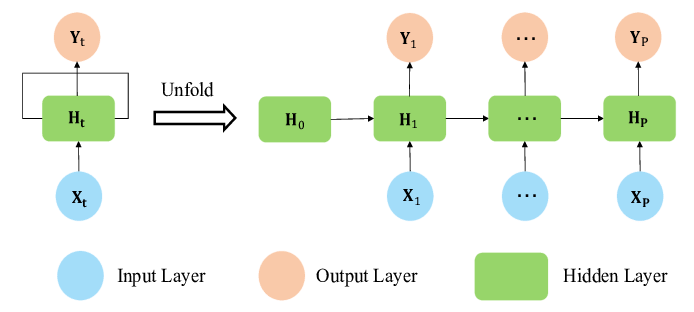
\includegraphics[width=10cm]{images/rnn3.png}
    \label{fig:fig6}
    \caption{The folded and unfolded structure of recurrent neural networks, \href{https://www.researchgate.net/figure/The-folded-and-unfolded-structure-of-recurrent-neural-networks-1-RNN-Similar-to-a_fig5_341639694}{source}}
    \end{figure}

}

\frame{\frametitle{Fake Wikipedia Page!}

	\begin{figure}
	\centering
    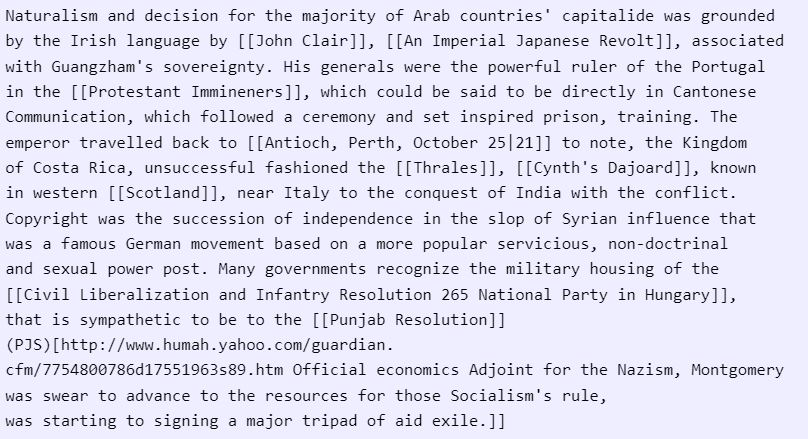
\includegraphics[width=11.5cm]{images/wikipedia.JPG}
    \label{fig:fig1}
    \caption{In case you were wondering, the yahoo url in the generated Wikipedia page doesn’t actually exist, the model just hallucinated it.}
    \end{figure}

}

\frame{\frametitle{Fake Algebraic Geometry Book!}
\begin{figure}
	\centering
    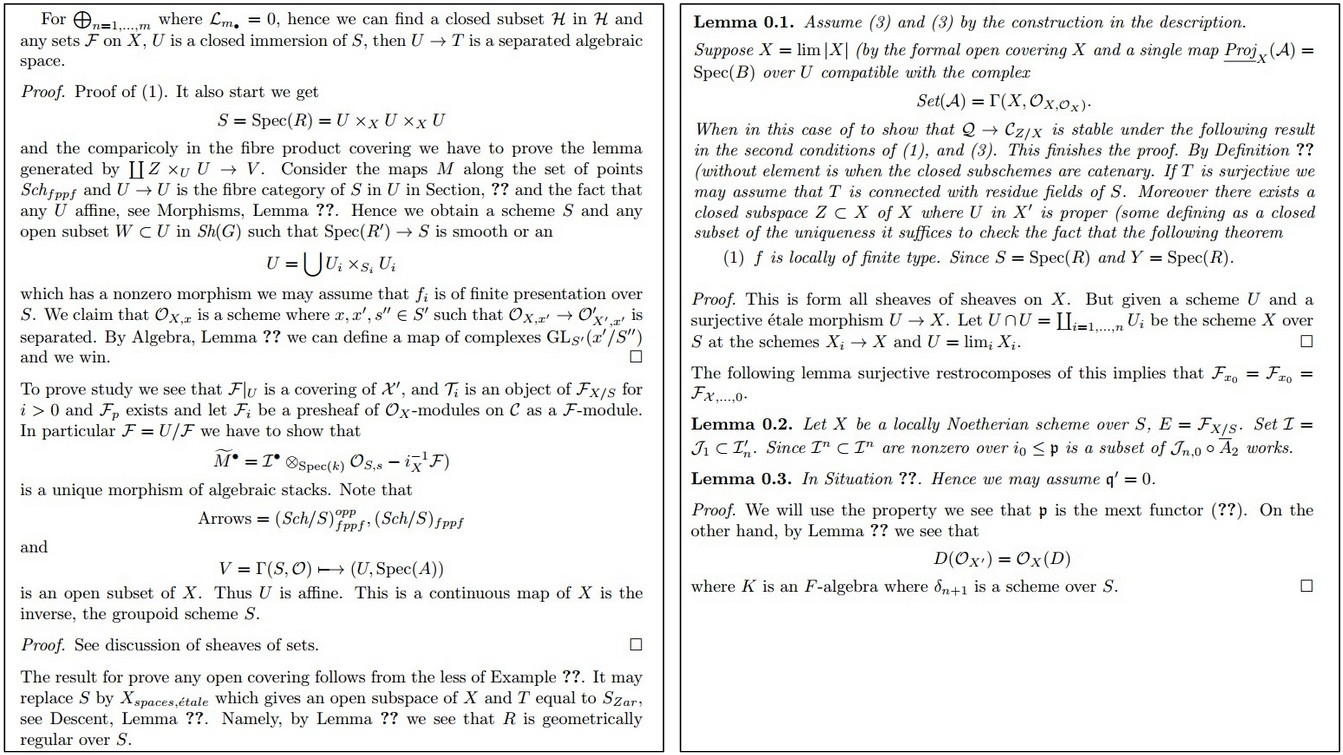
\includegraphics[width=11.5cm]{images/algebric.jpeg}
    \label{fig:fig2}
    \caption{A sample of a recurrent network. The network is trained on the raw Latex source file of a book on algebraic geometry. Amazingly, the resulting sampled Latex almost compiles!}
    \end{figure}
}


\frame{\frametitle{Fake C Code!}
\begin{figure}
	\centering
    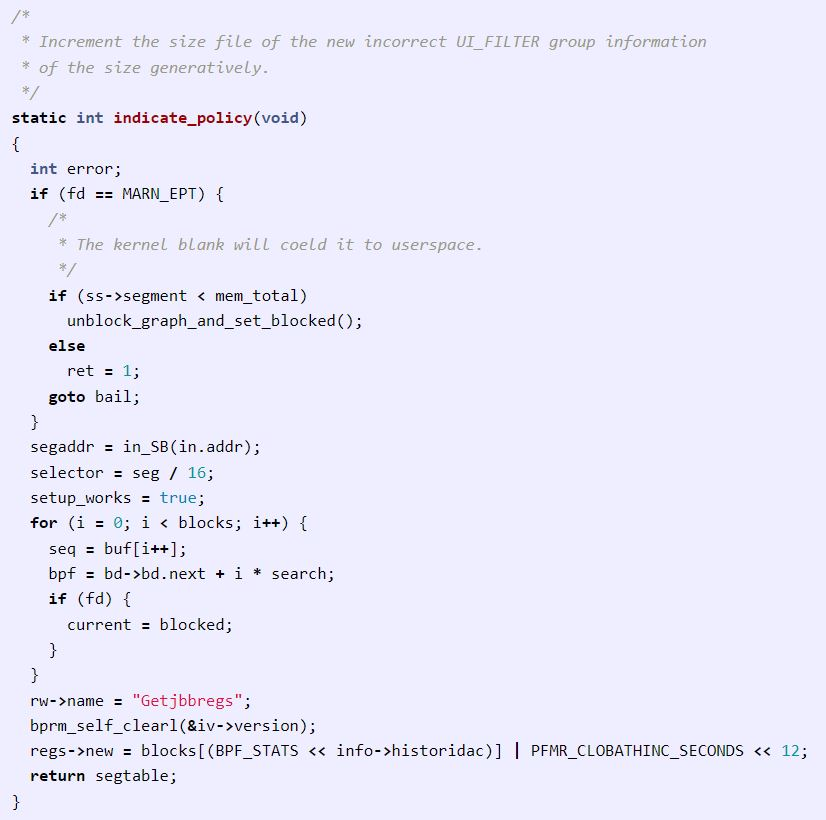
\includegraphics[width=6.8cm]{images/c.jpg}
    \label{fig:fig3}
    \caption{This time the network is trained on the linux source code. Notice the comments, pointer notation and brackets in the above code. What are the code errors?}
\end{figure}
}

\frame{\frametitle{The Effectiveness of Recurrent Neural Networks}
\begin{itemize}
    \item All previous examples were generated blindly by recurrent neural network with simple architectures.
    \vspace{5mm}
    \item Interested? Take a look at the source: \href{http://karpathy.github.io/2015/05/21/rnn-effectiveness/}{ http://karpathy.github.io/2015/05/21/rnn-effectiveness/}
\end{itemize}
}


\frame{\frametitle{Modeling Series}
\begin{itemize}
\item In many situations one must consider a series of inputs to produce an output.
    \begin{itemize}
    \item Outputs too may be a series
    \end{itemize}
\vspace{5mm}
\item Examples...?
\end{itemize}
}

\frame{\frametitle{Example 1: Speech Recognition}
\begin{figure}
	\centering
    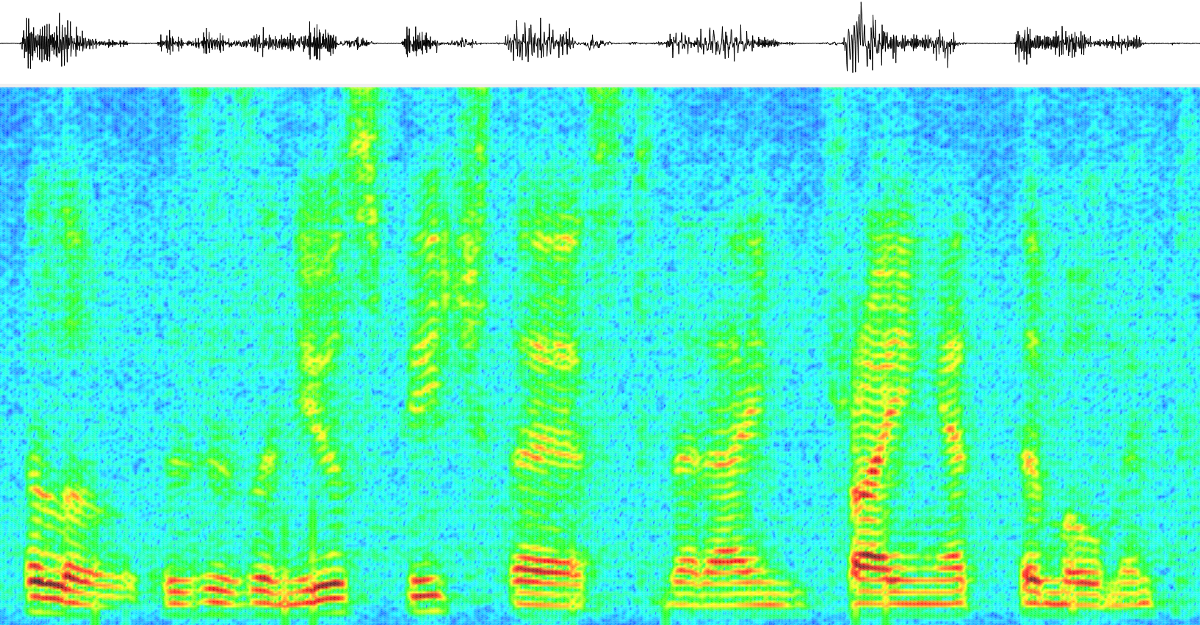
\includegraphics[width=9cm]{images/spectral.png}
    \label{fig:fig4}
    \caption{\href{https://towardsdatascience.com/recognizing-speech-commands-using-recurrent-neural-networks-with-attention-c2b2ba17c837}{source}}
\end{figure}
\begin{itemize}
\item Speech Recognition
    \begin{itemize}
    \item Analyze a series of spectral vectors, determine what was said.
    \end{itemize}
\vspace{2mm}
\item Note: Inputs are sequences of vectors. Output is a classification result.
\vspace{5mm}
\end{itemize}
}

\frame{\frametitle{Example 2: Text Analysis}
\begin{tcolorbox}
\textit{Stephen Curry scored 34 points and was named the NBA Finals MVP as the Warriors claimed the franchise’s seventh championship overall. And this one completed a journey like none other, after a run of five consecutive finals, then a plummet to the bottom of the NBA, and now a return to greatness just two seasons after having the league’s worst record.}
\end{tcolorbox}

\begin{itemize}
\item Football or Basketball?
\vspace{5mm}
\item Text Analysis
\vspace{2mm}
    \begin{itemize}
    \item E.g. analyze document, identify topic
        \begin{itemize}
            \item Input series of words, output classification output
        \end{itemize}
\vspace{2mm}
    \item E.g. read English, output Persian
        \begin{itemize}
            \item Input series of words, output series of words
        \end{itemize}
    \end{itemize}
\vspace{1mm}
\end{itemize}
}


\frame{\frametitle{Example 3: Stock Market Prediction}
\begin{figure}
	\centering
    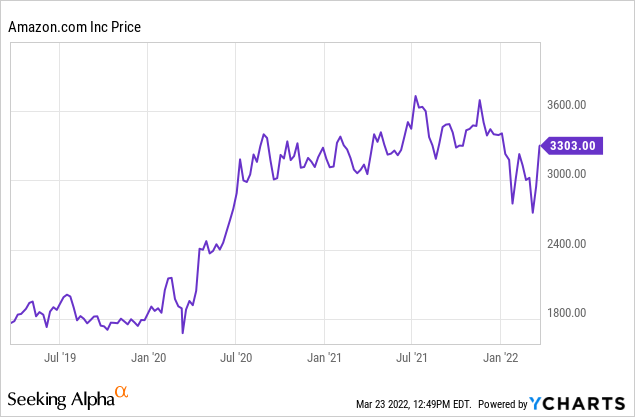
\includegraphics[width=8cm]{images/amazon.png}
    \label{fig:fig5}
\end{figure}
\begin{itemize}
\item Stock Market Prediction
    \begin{itemize}
    \item Should I invest, vs. should I not invest in X?
    \item Decision must be taken considering how things have fared over time.
    \end{itemize}
\vspace{2mm}
\item Note: Inputs are sequences of vectors. Output may be 
scalar or vector.
\vspace{2mm}
\end{itemize}
}

\frame{\frametitle{Stock Market Prediction}
\begin{figure}
	\centering
    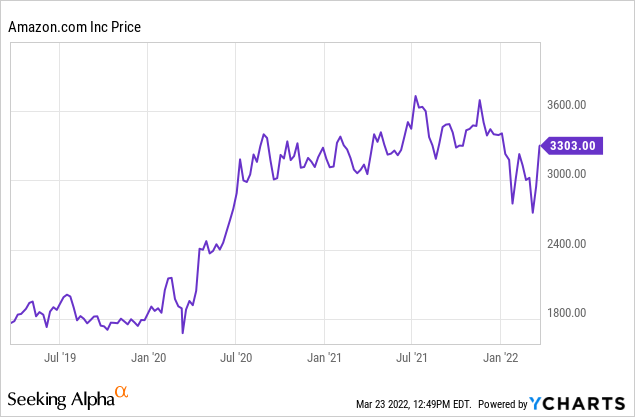
\includegraphics[width=8cm]{images/amazon.png}
    \label{fig:fig5}
\end{figure}
\begin{itemize}
\item Stock Market Prediction
    \begin{itemize}
    \item Must consider the series of stock values several days in the past to decide
    \item How should we design our network?
    \end{itemize}
\vspace{2mm}
\end{itemize}
}

\frame{\frametitle{The Stock Predictor Network}
\vspace{-5mm}
\begin{figure}
	\centering
    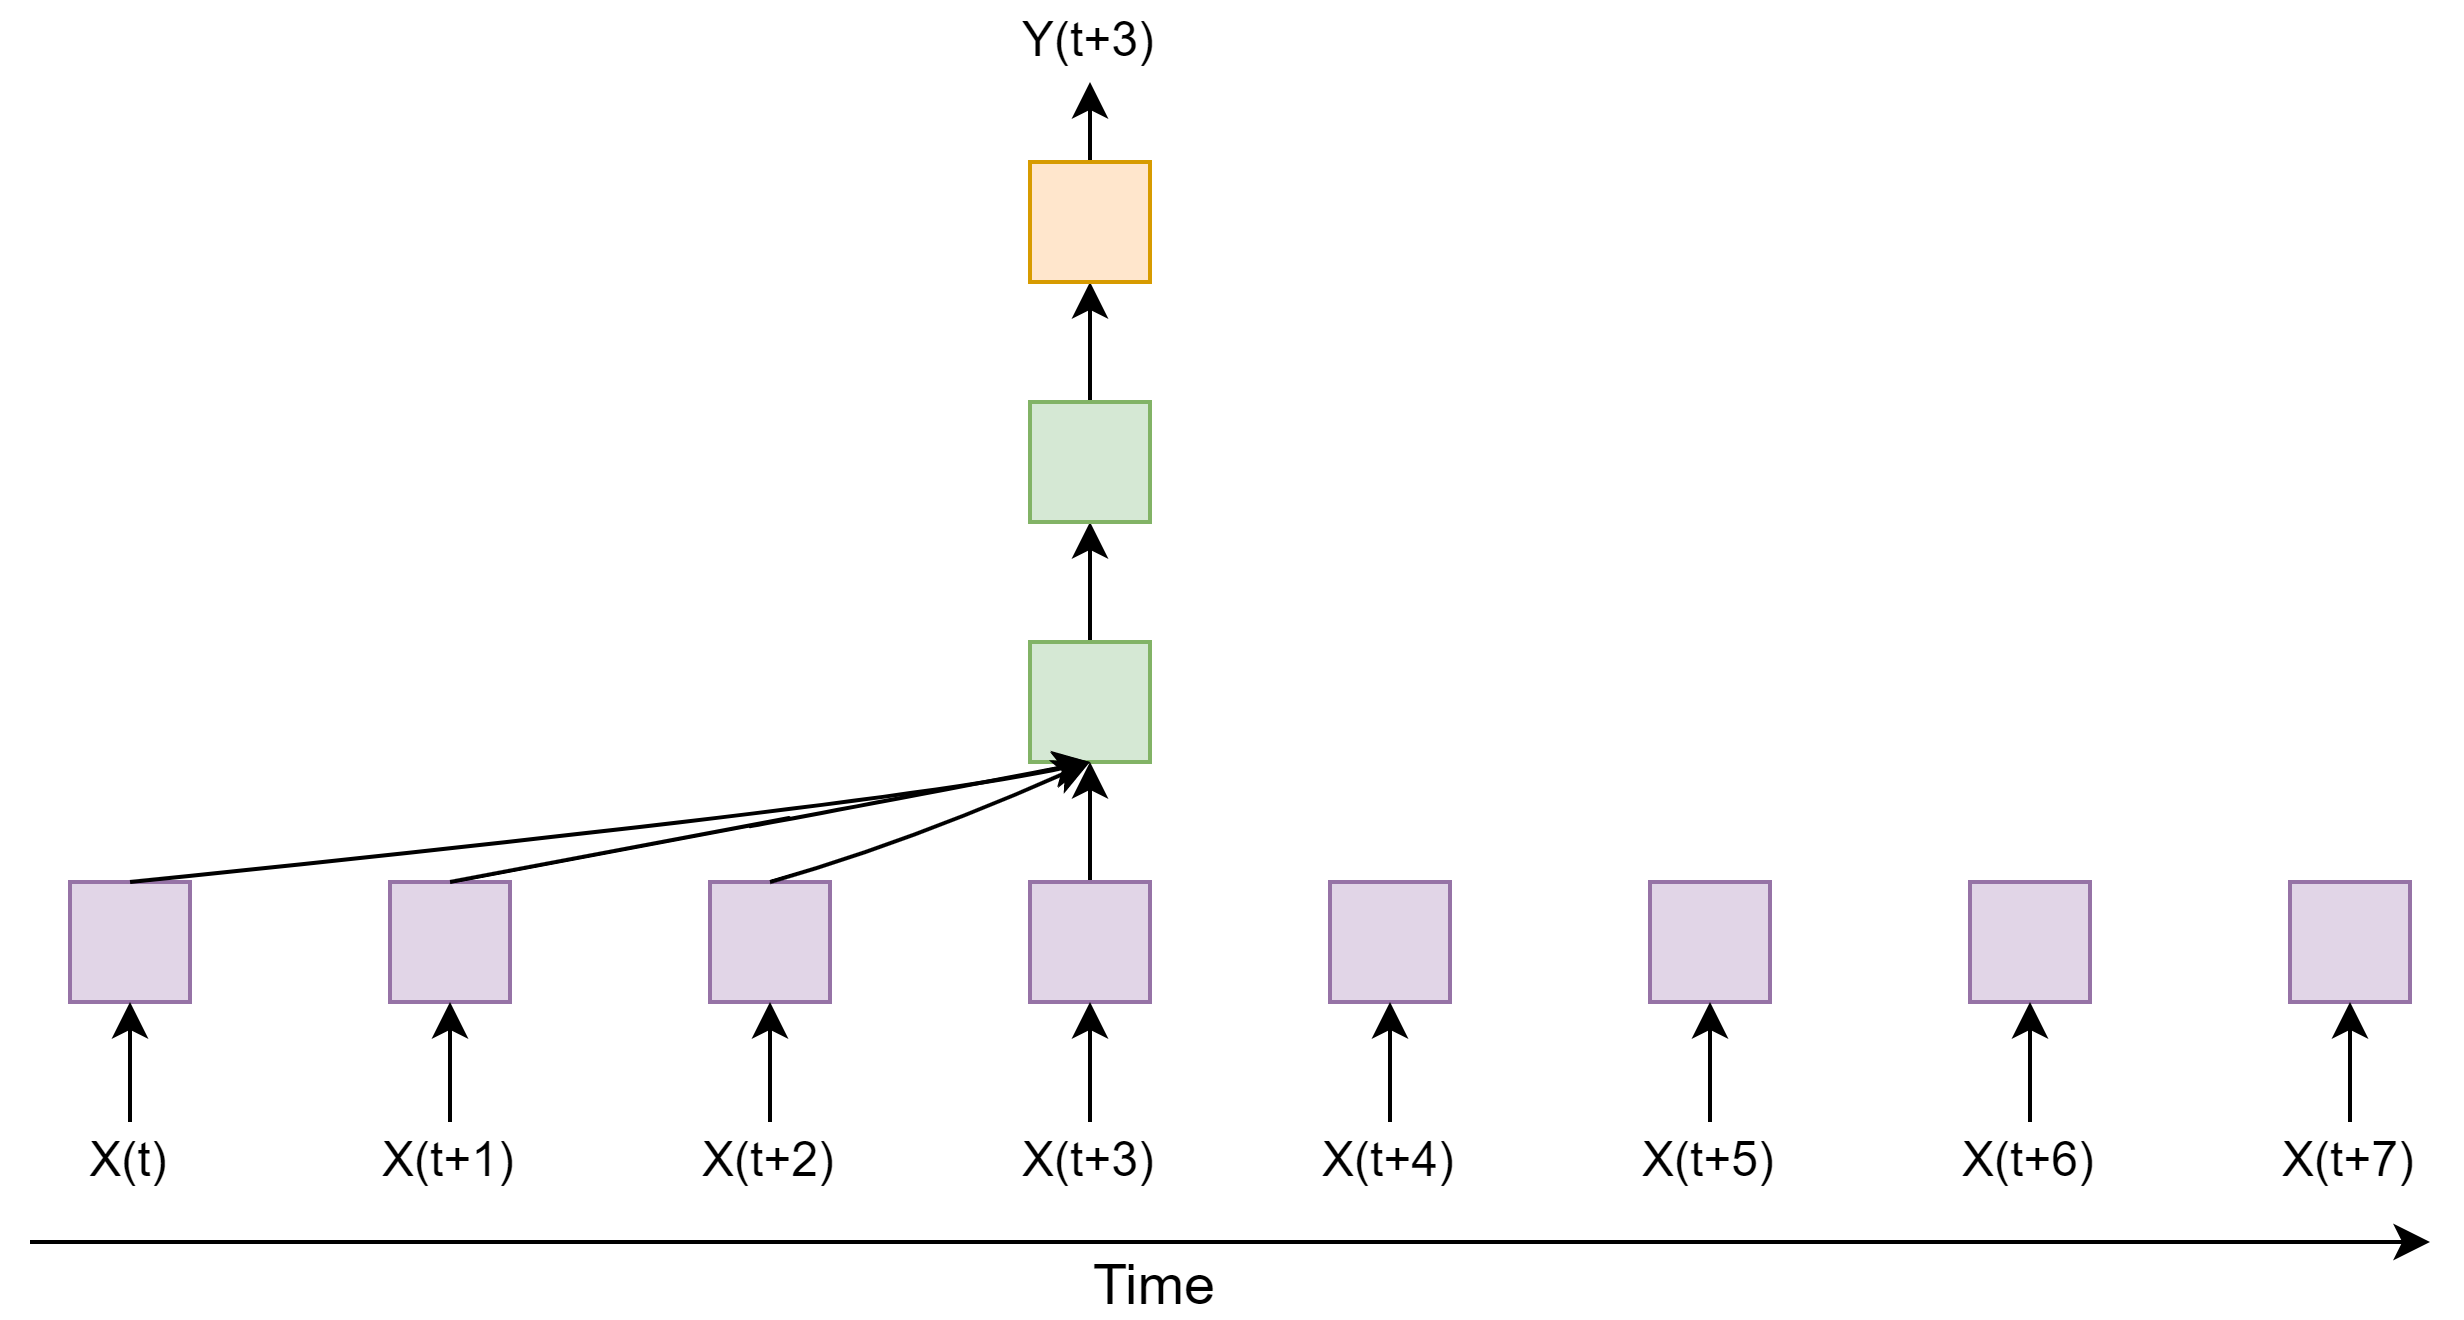
\includegraphics[width=9.5cm, height=5cm]{images/market_network1.png}
    \label{fig:fig7}
\end{figure}
\vspace{-8mm}
\begin{itemize}
\item The sliding predictor
    \begin{itemize}
    \item Look at the last few days
    \item This is just an CNN applied to series data
    \begin{itemize}
        \item Also called a Time-Delay neural network
    \end{itemize}
    \end{itemize}
\item Representational shortcut
    \begin{itemize}
        \item Input at each time is a vector
        \item Each box actually represents an entire layer with many units
    \end{itemize}
\end{itemize}
}

\frame{\frametitle{The Stock Predictor Network}
\vspace{-5mm}
\begin{figure}
	\centering
    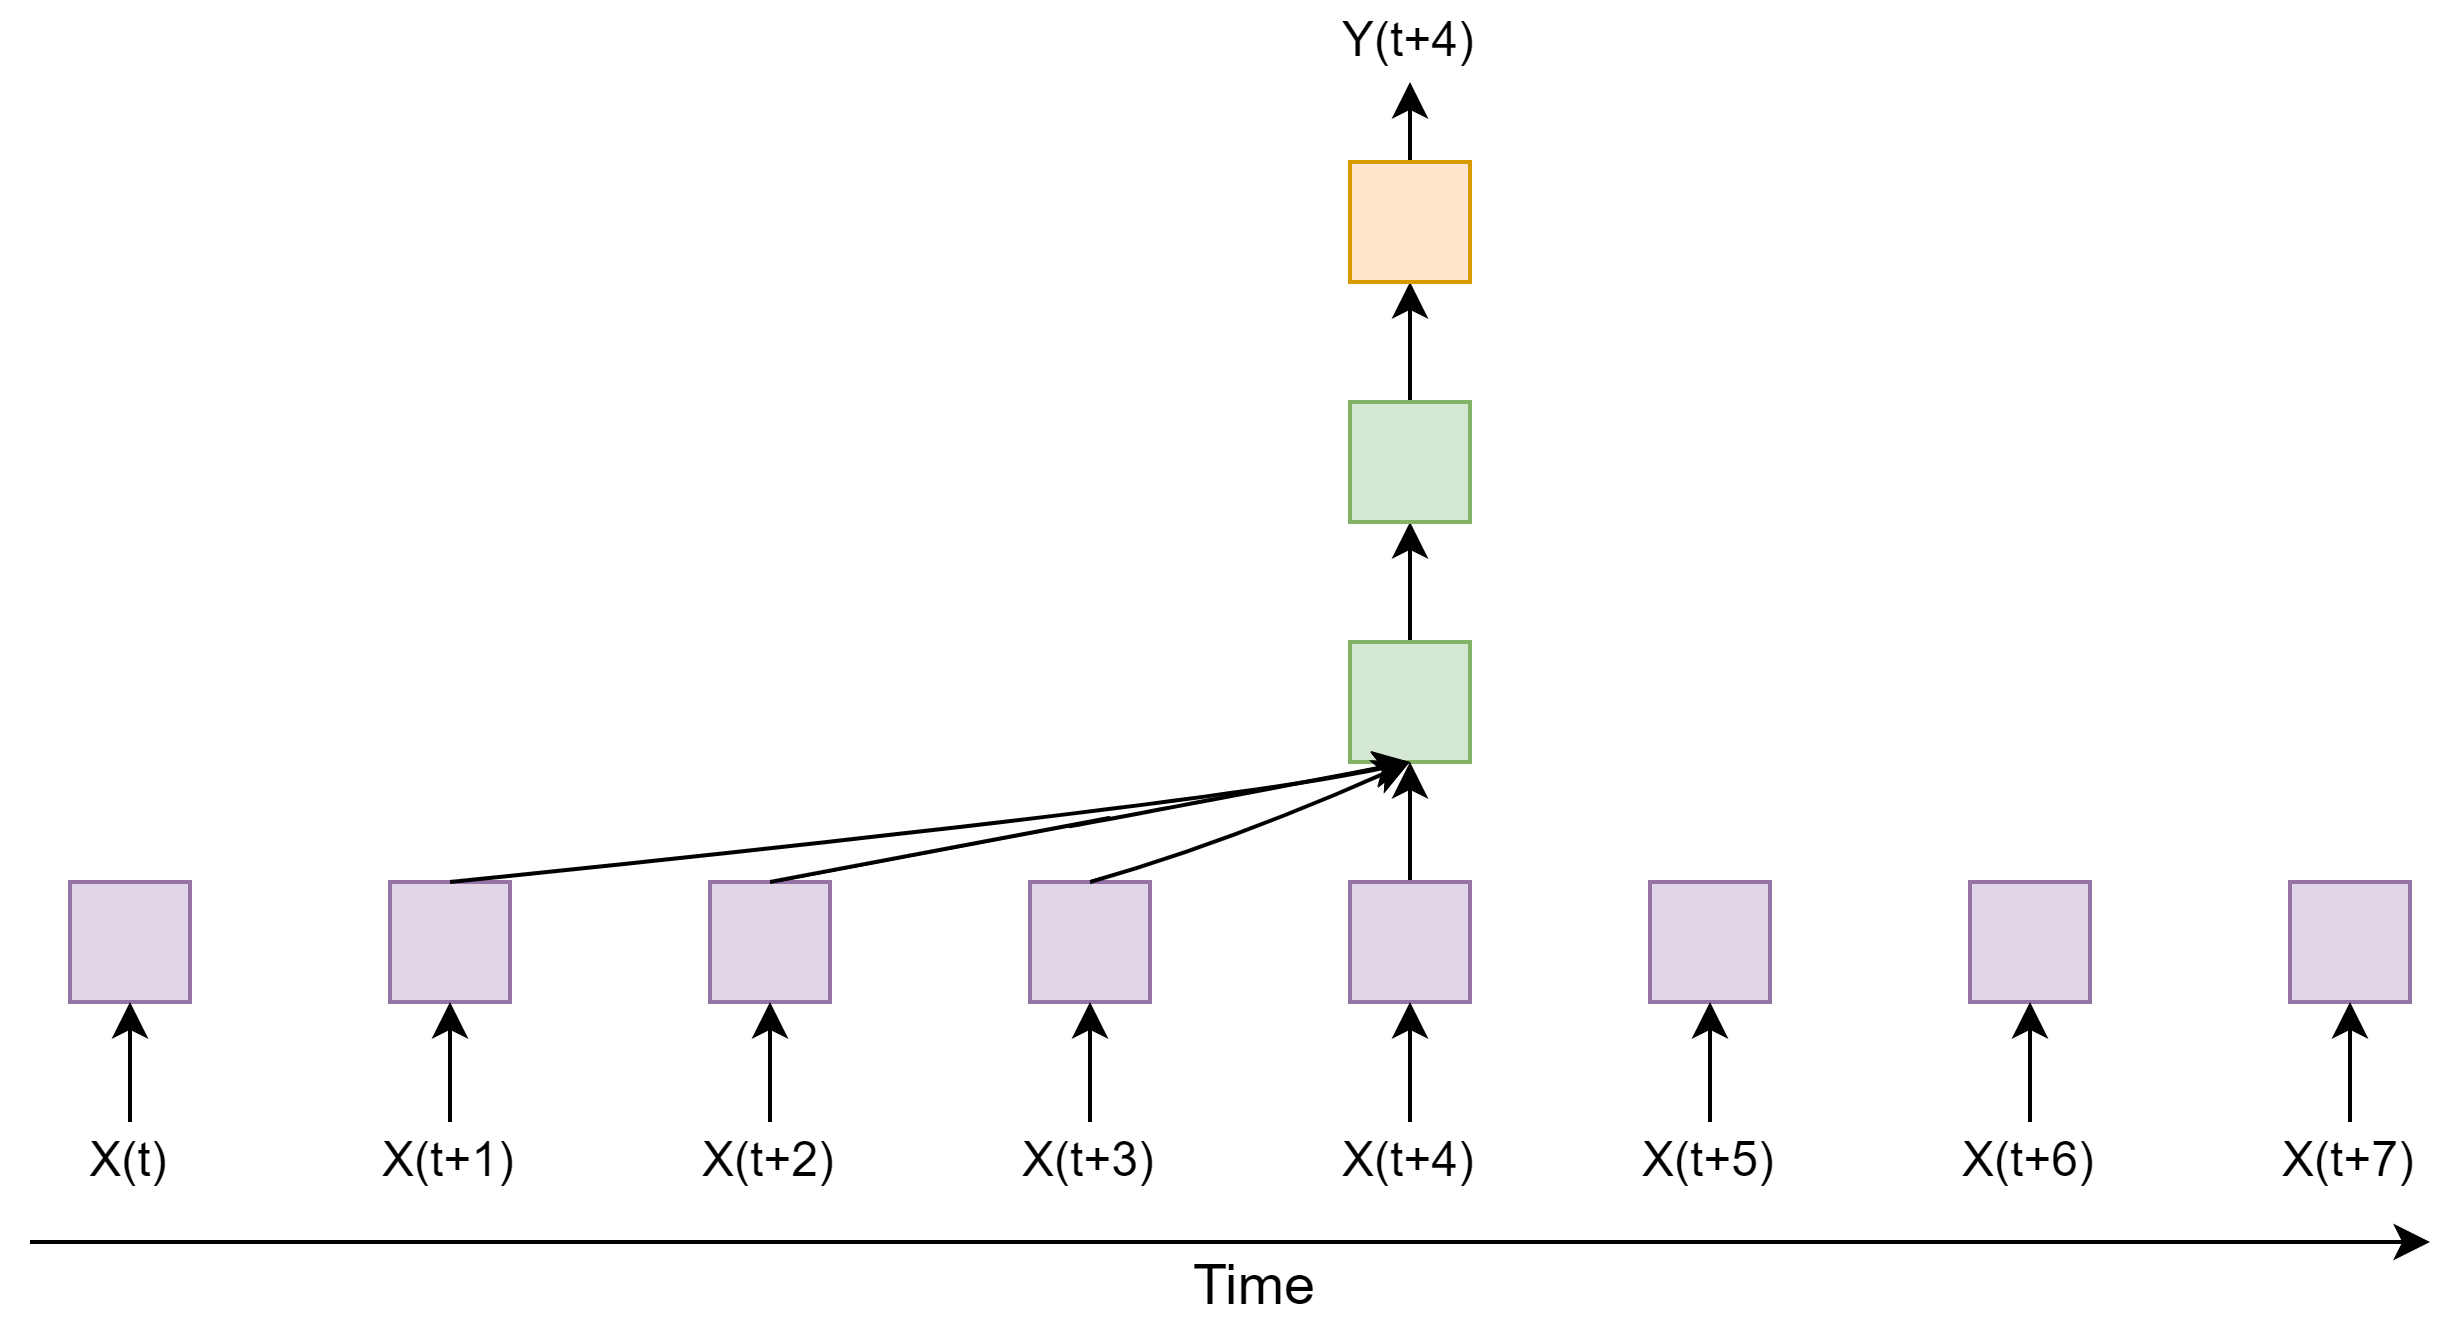
\includegraphics[width=9.5cm, height=5cm]{images/market_network2.png}
    \label{fig:fig7}
\end{figure}
\vspace{-8mm}
\begin{itemize}
\item The sliding predictor
    \begin{itemize}
    \item Look at the last few days
    \item This is just an CNN applied to series data
    \begin{itemize}
        \item Also called a Time-Delay neural network
    \end{itemize}
    \end{itemize}
\item Representational shortcut
    \begin{itemize}
        \item Input at each time is a vector
        \item Each box actually represents an entire layer with many units
    \end{itemize}
\end{itemize}
}

\frame{\frametitle{The Stock Predictor Network}
\vspace{-5mm}
\begin{figure}
	\centering
    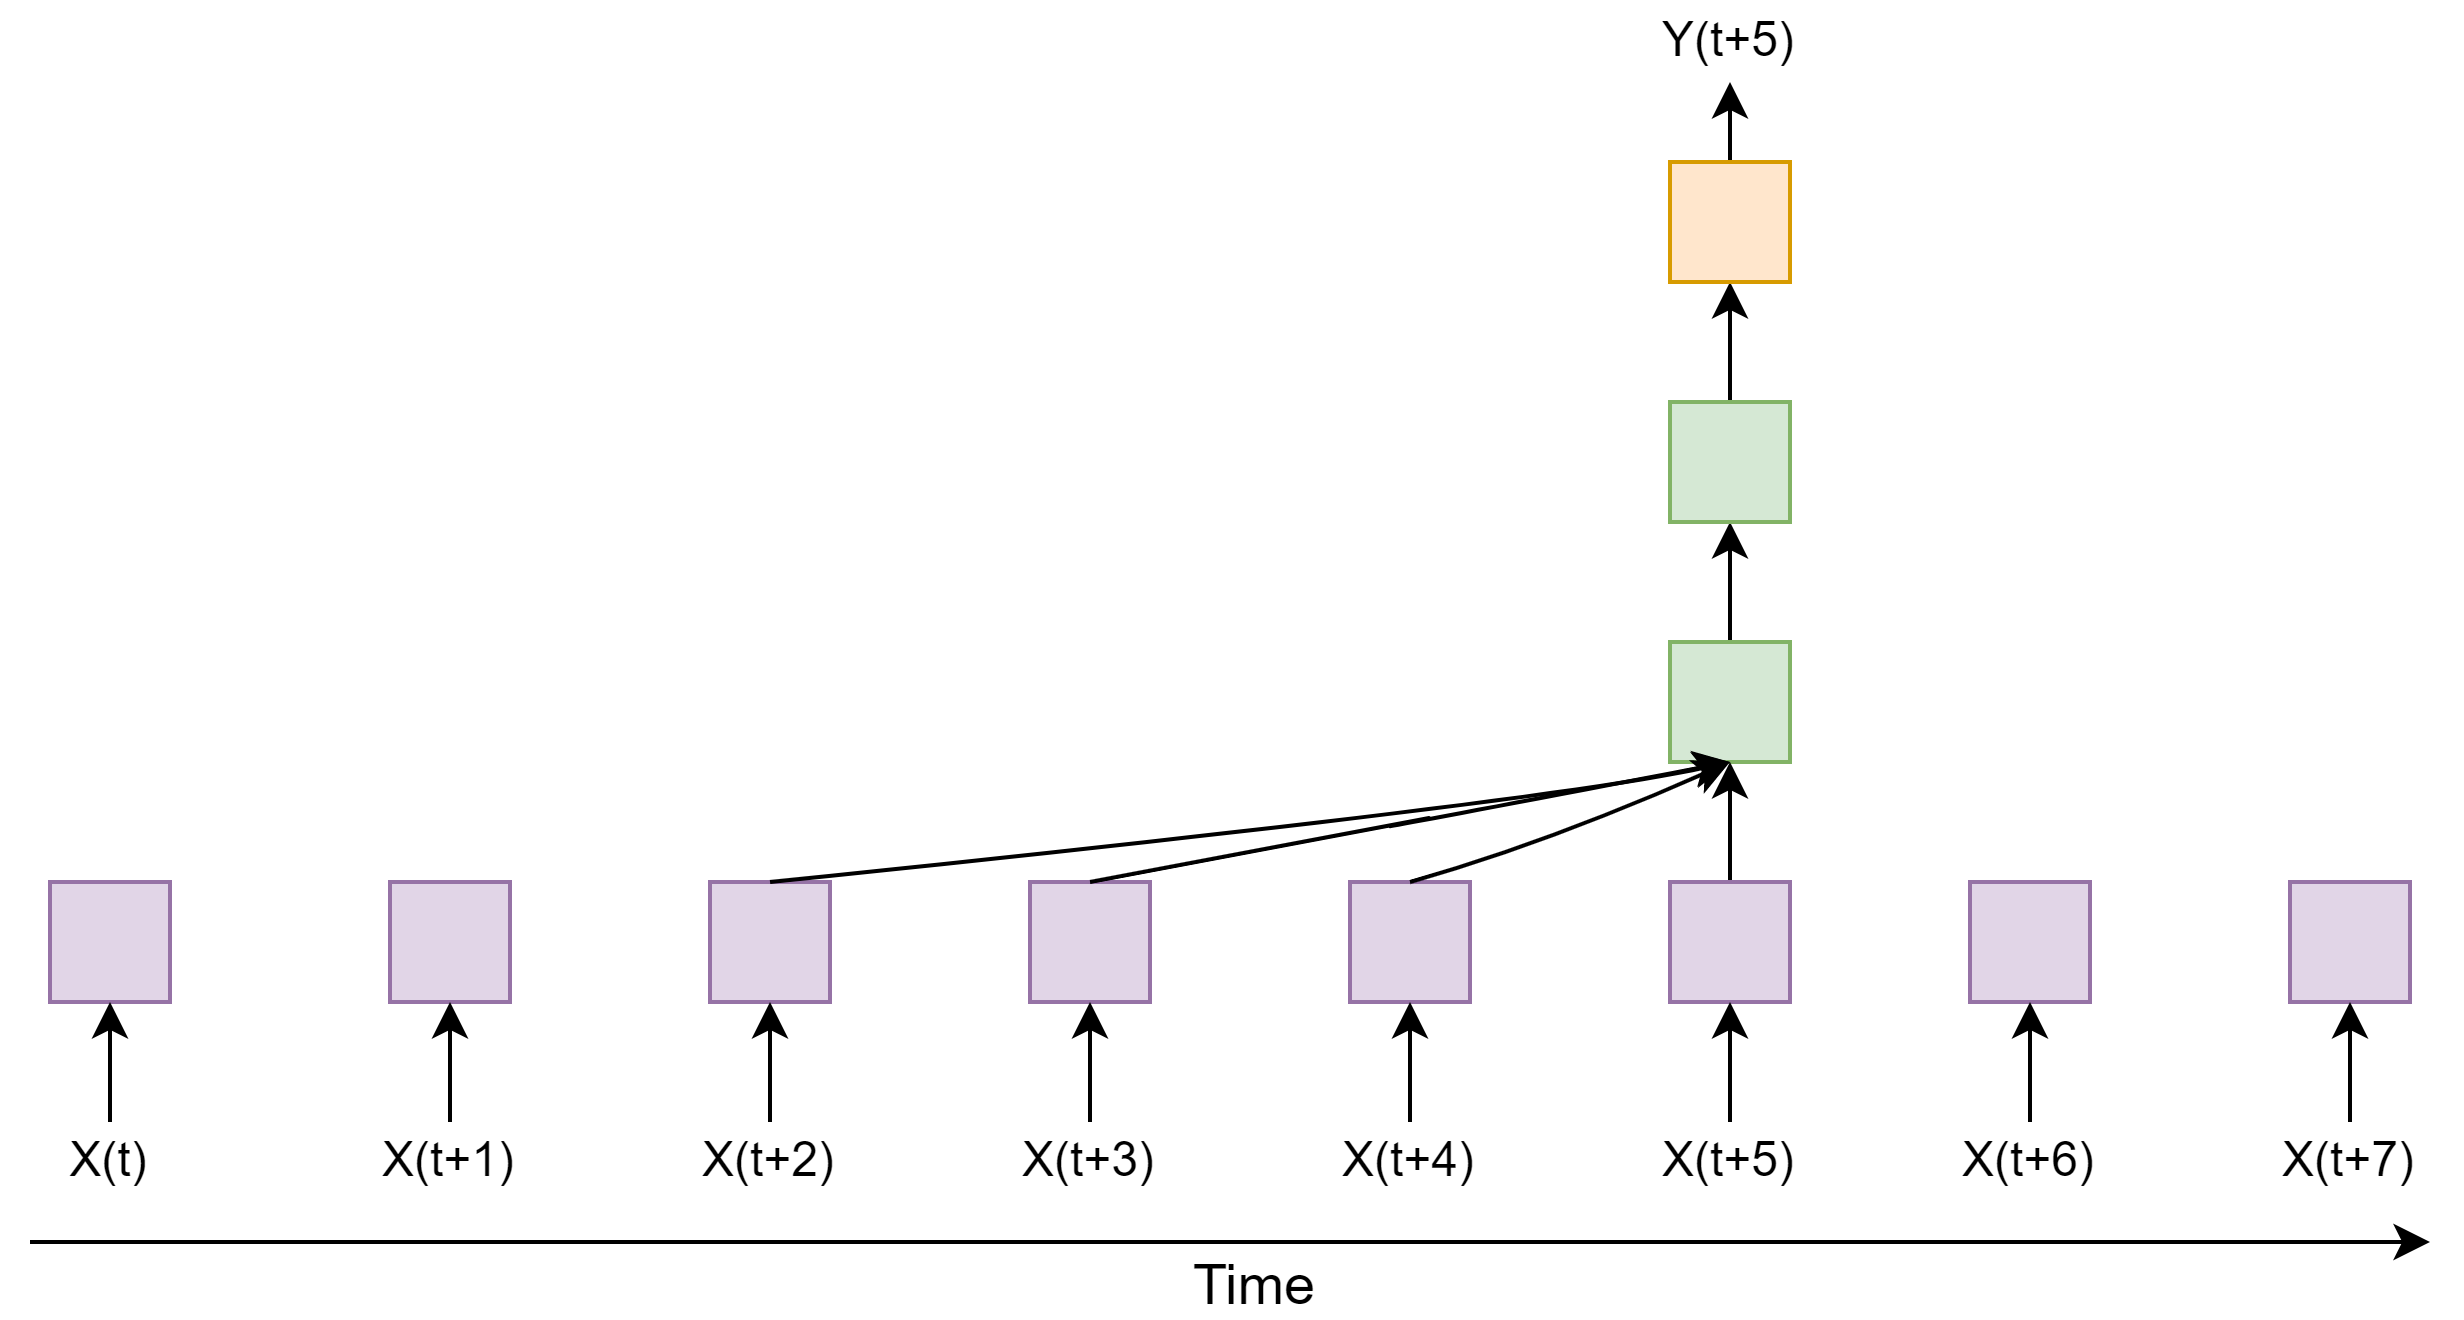
\includegraphics[width=9.5cm, height=5cm]{images/market_network3.png}
    \label{fig:fig7}
\end{figure}
\vspace{-8mm}
\begin{itemize}
\item The sliding predictor
    \begin{itemize}
    \item Look at the last few days
    \item This is just an CNN applied to series data
    \begin{itemize}
        \item Also called a Time-Delay neural network
    \end{itemize}
    \end{itemize}
\item Representational shortcut
    \begin{itemize}
        \item Input at each time is a vector
        \item Each box actually represents an entire layer with many units
    \end{itemize}
\end{itemize}
}

\frame{\frametitle{The Stock Predictor Network}
\vspace{-5mm}
\begin{figure}
	\centering
    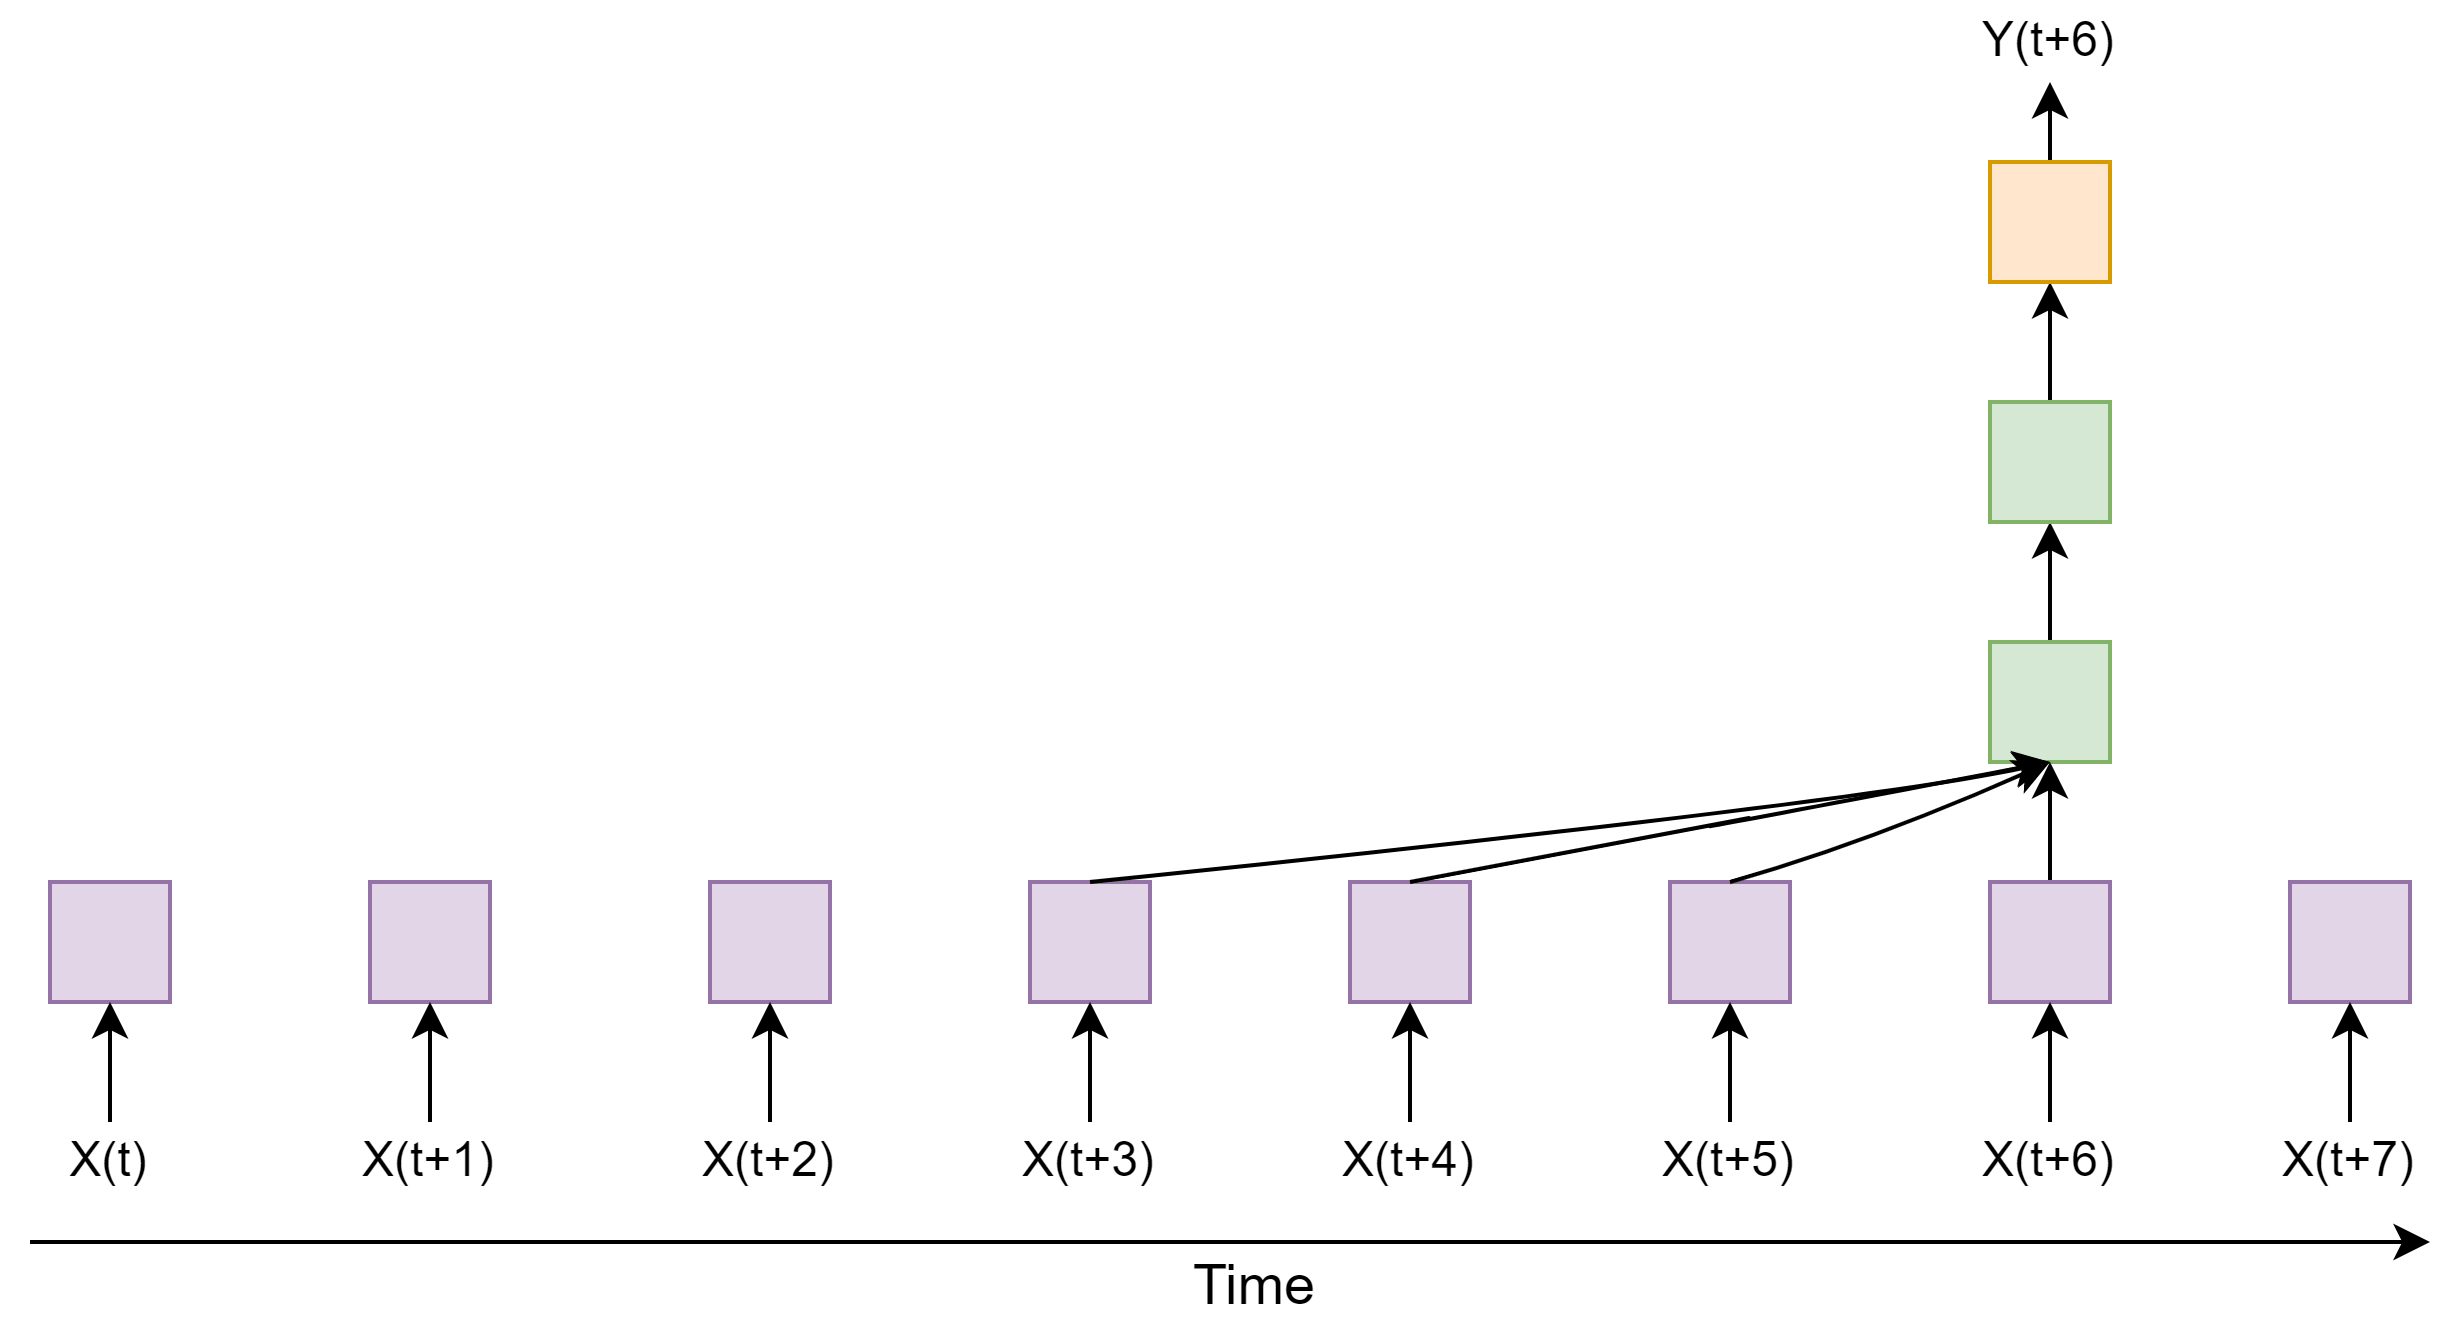
\includegraphics[width=9.5cm, height=5cm]{images/market_network4.png}
    \label{fig:fig7}
\end{figure}
\vspace{-8mm}
\begin{itemize}
\item The sliding predictor
    \begin{itemize}
    \item Look at the last few days
    \item This is just an CNN applied to series data
    \begin{itemize}
        \item Also called a Time-Delay neural network
    \end{itemize}
    \end{itemize}
\item Representational shortcut
    \begin{itemize}
        \item Input at each time is a vector
        \item Each box actually represents an entire layer with many units
    \end{itemize}
\end{itemize}
}

\frame{\frametitle{Finite Response Model}
\vspace{-5mm}
\begin{figure}
	\centering
    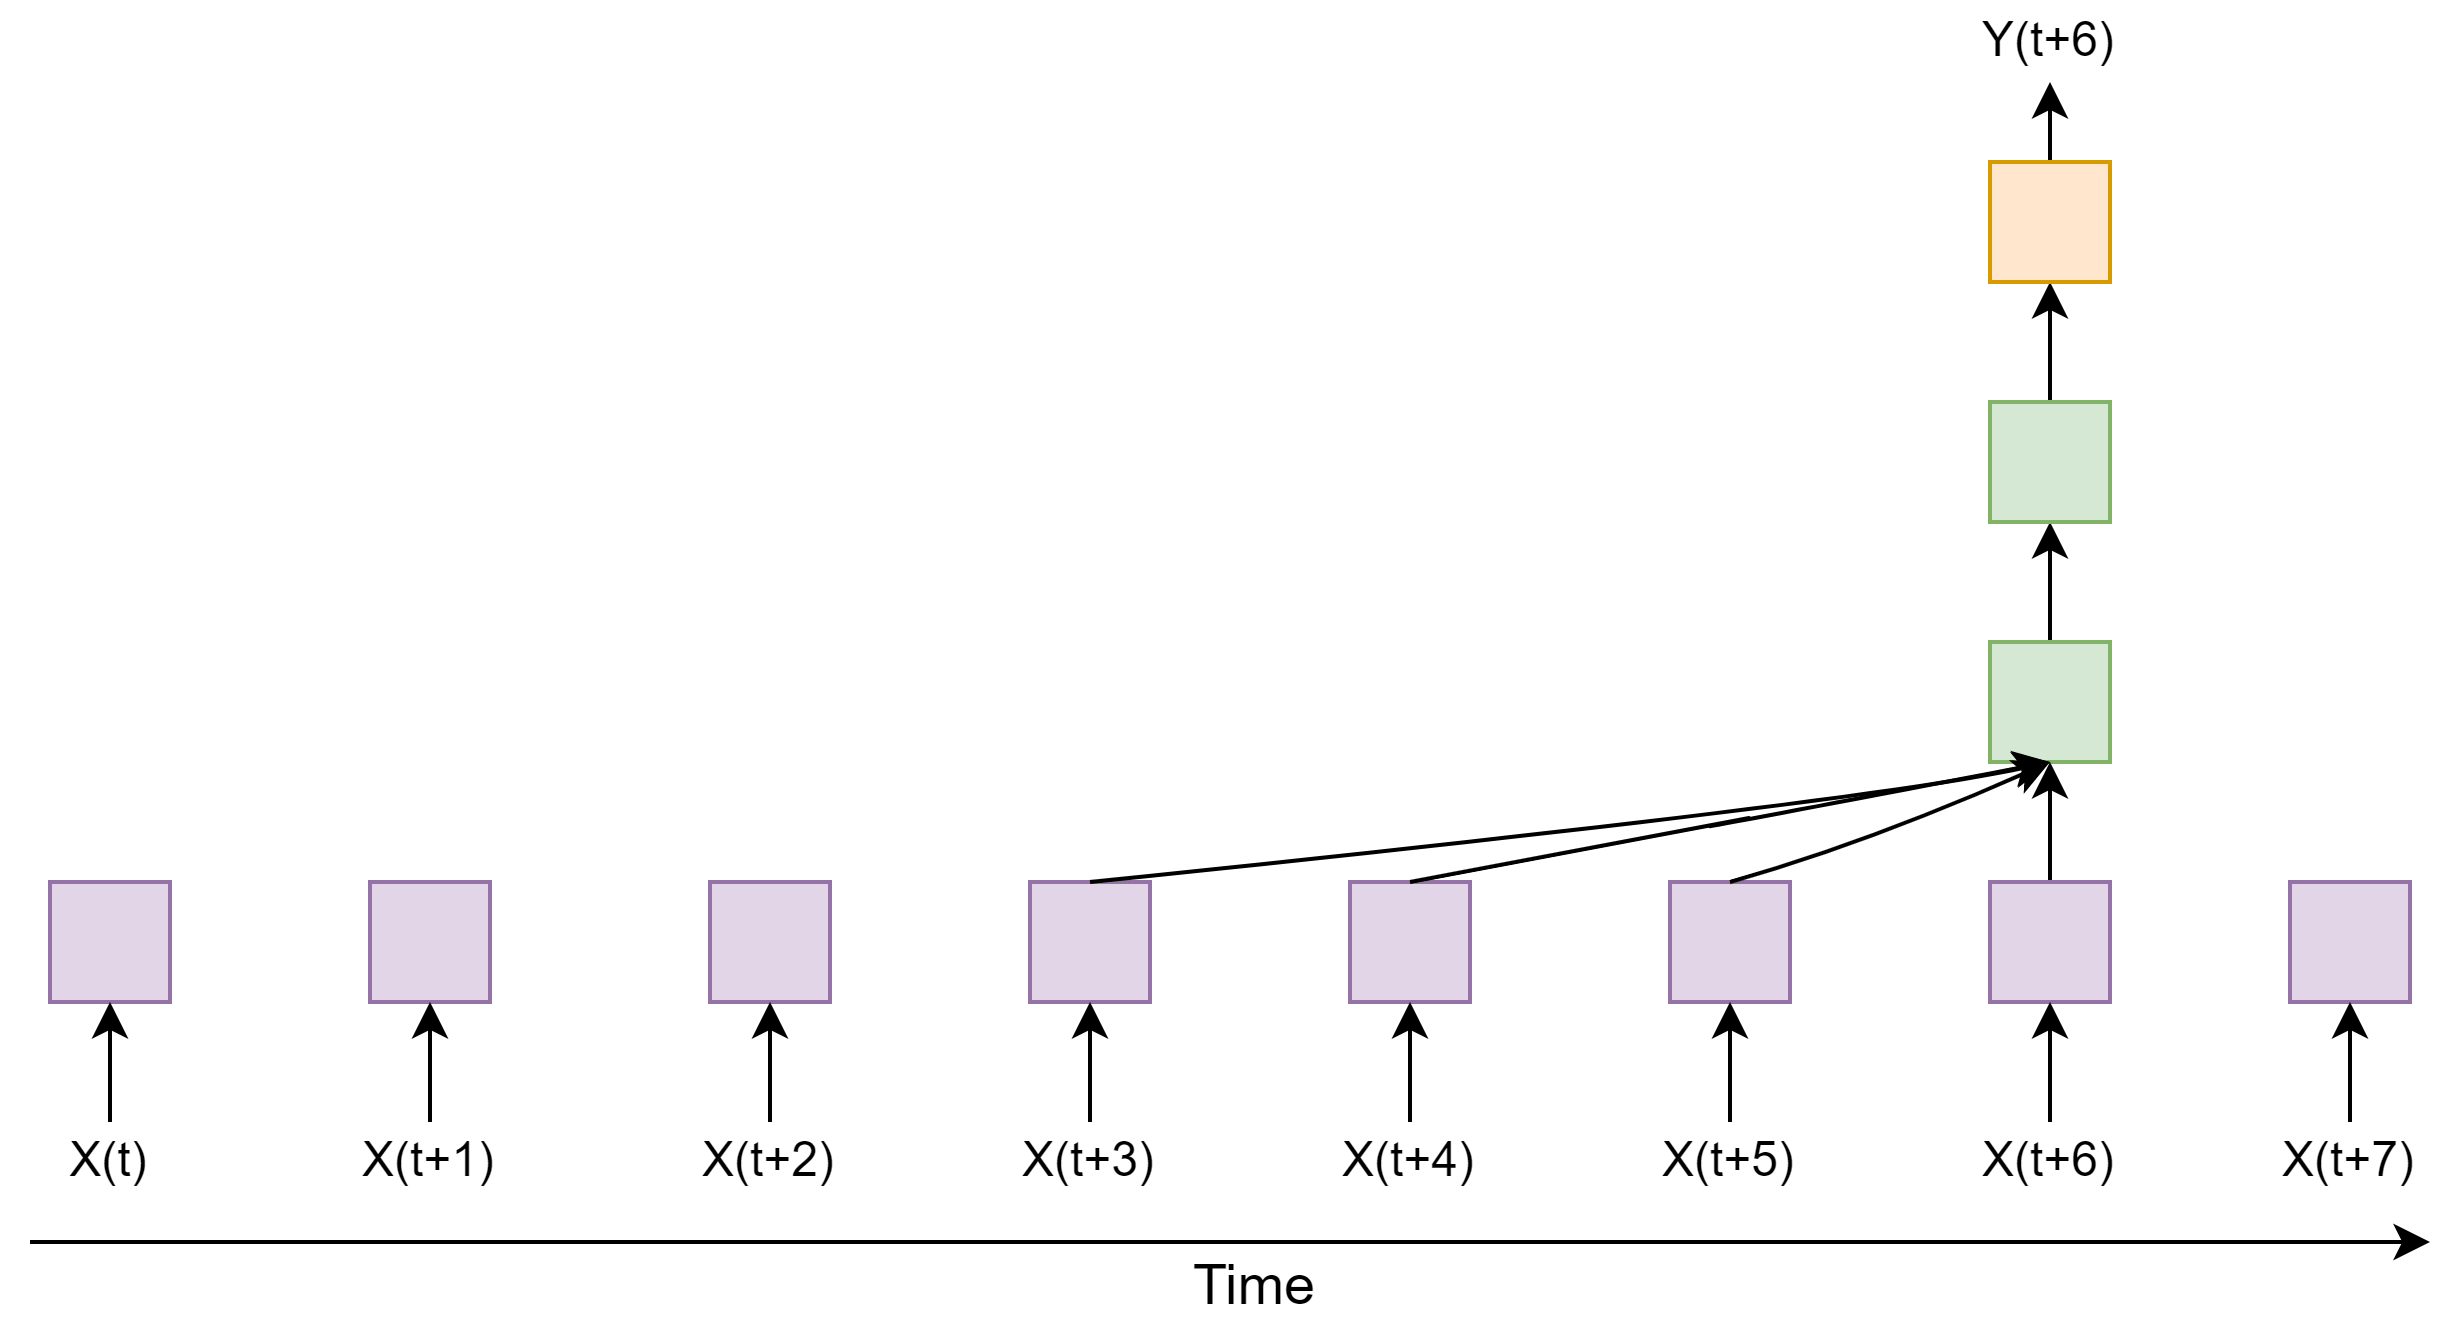
\includegraphics[width=9.5cm, height=5cm]{images/market_network4.png}
    \label{fig:fig7}
\end{figure}
\begin{itemize}
\item This is a finite response system
    \begin{itemize}
    \item Something that happens today only affects the output of the system for $N$ days into the future
    \begin{itemize}
        \item $N$ is the width of the system
    \end{itemize}
    \item $Y_t = f(X_t, X_{t-1},...,X_{t-N})$
    \end{itemize}
\end{itemize}
}

\frame{\frametitle{Finite Response Model}
\vspace{-5mm}
\begin{figure}
	\centering
    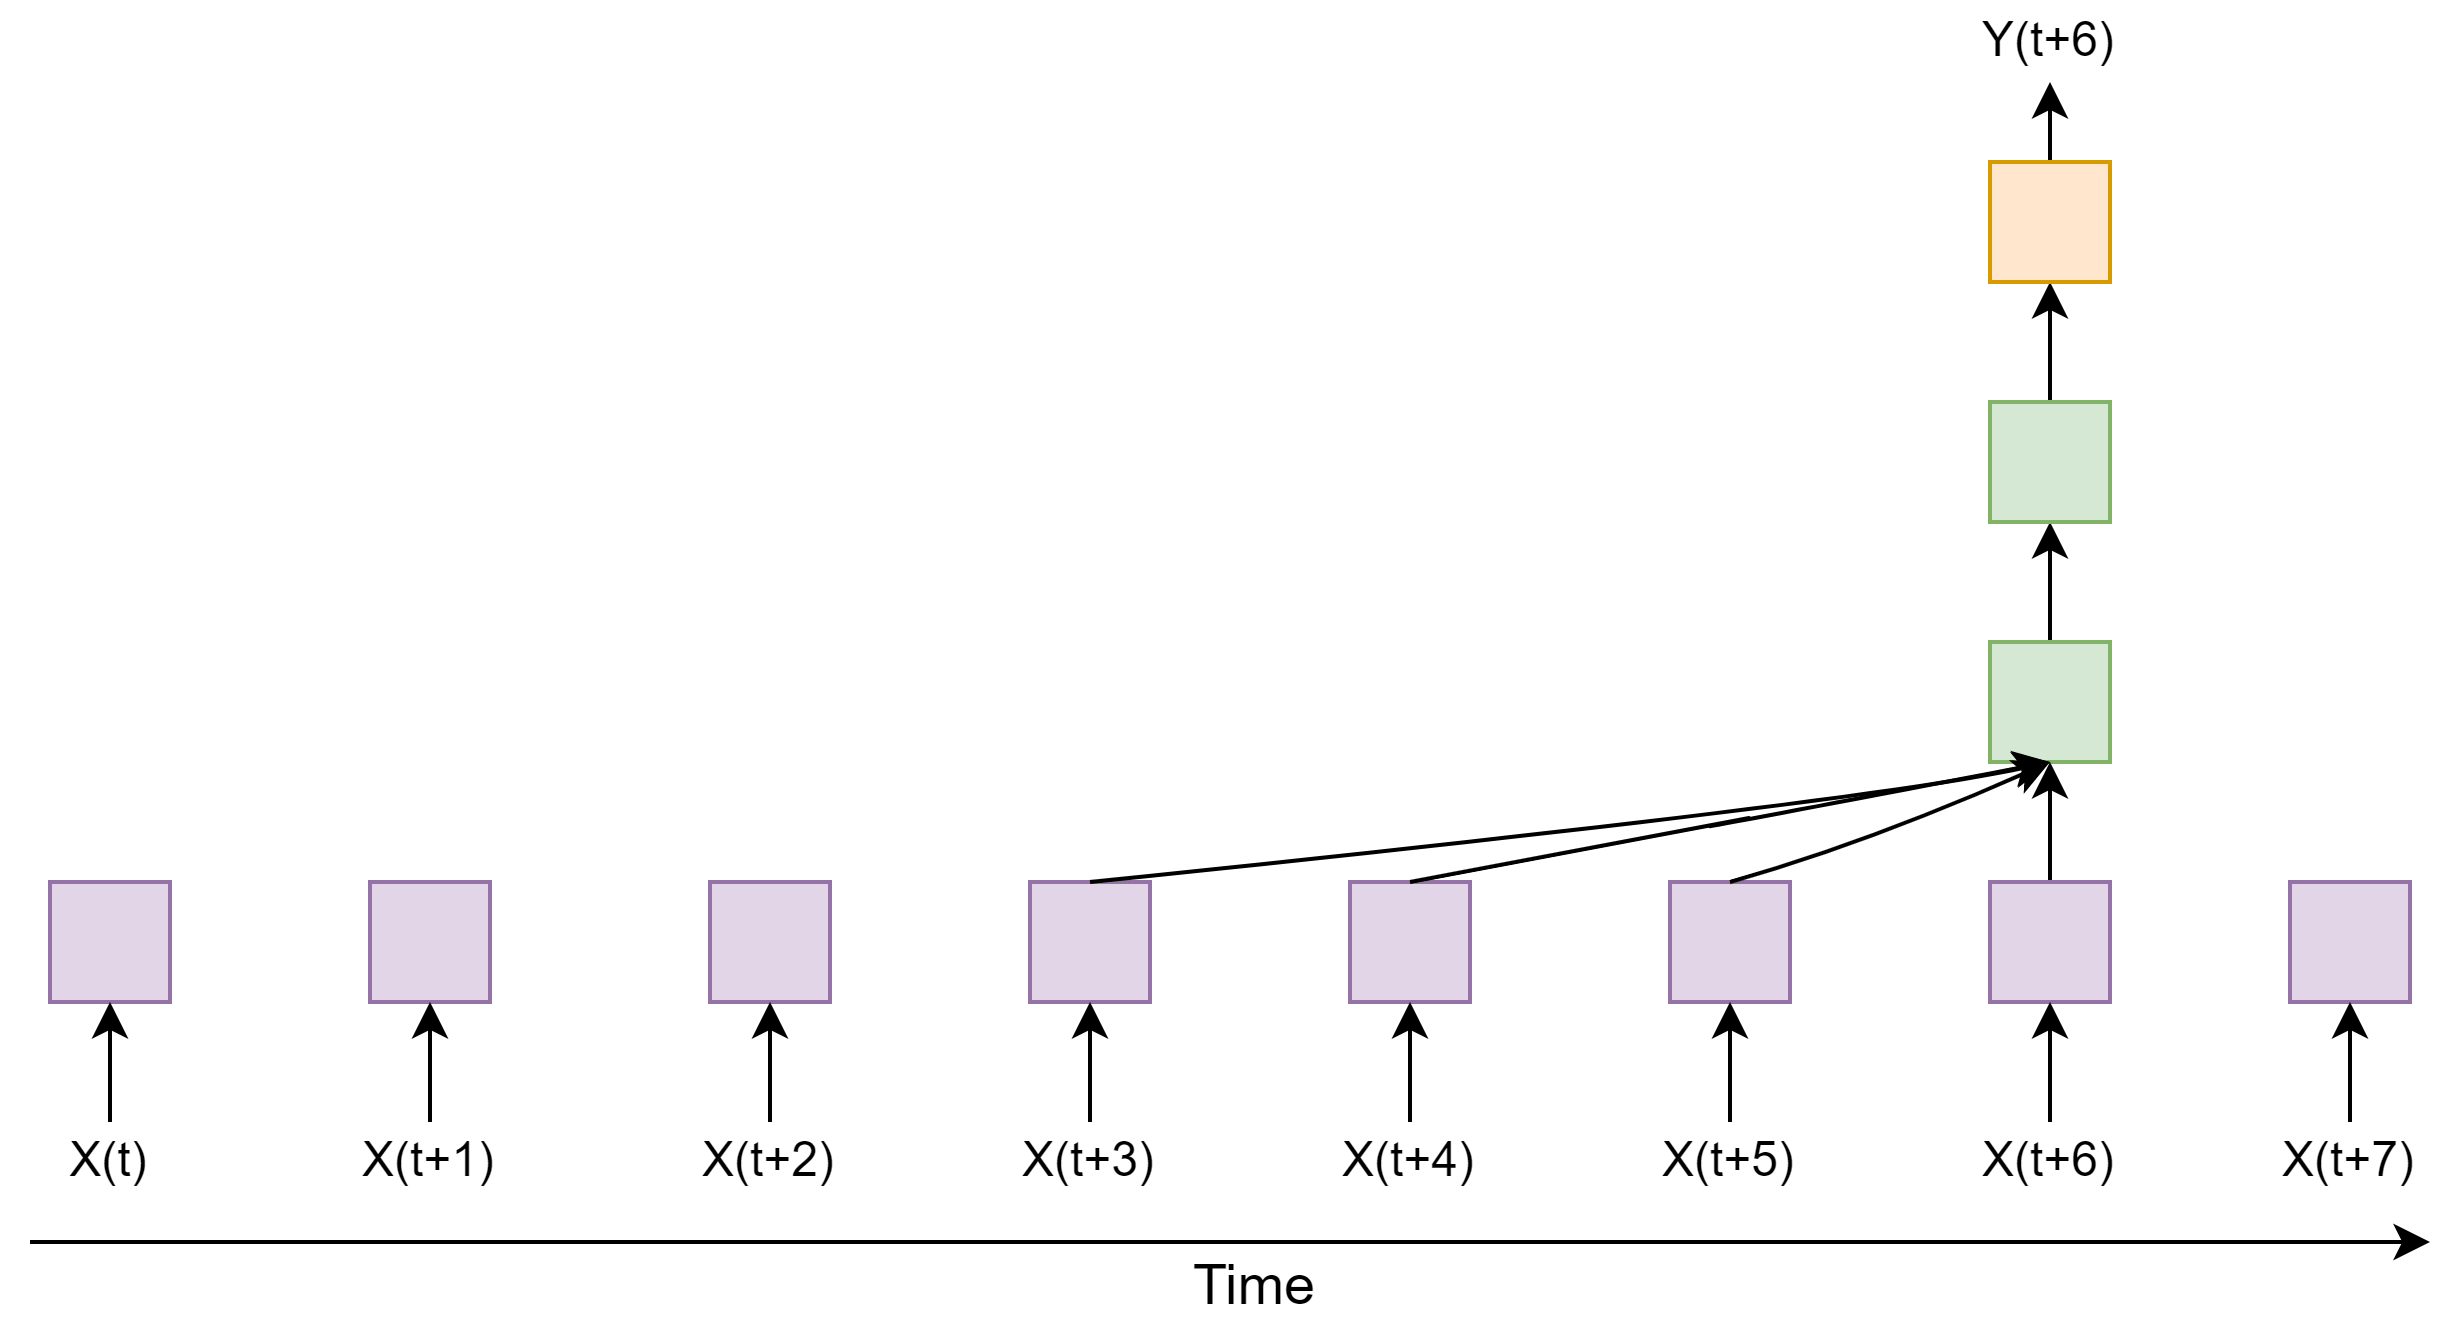
\includegraphics[width=9.5cm, height=5cm]{images/market_network4.png}
    \label{fig:fig7}
\end{figure}
\begin{itemize}
\item Something that happens today only affects the output of the
system for days into the future
    \begin{itemize}
    \item Predictions consider N days of history
    \end{itemize}
\item What if we need to consider more of the past to make predictions?
    \begin{itemize}
        \item Increase the “history”
    \end{itemize}
\end{itemize}
}

\frame{\frametitle{Finite Response Model}
\vspace{-5mm}
\begin{figure}
	\centering
    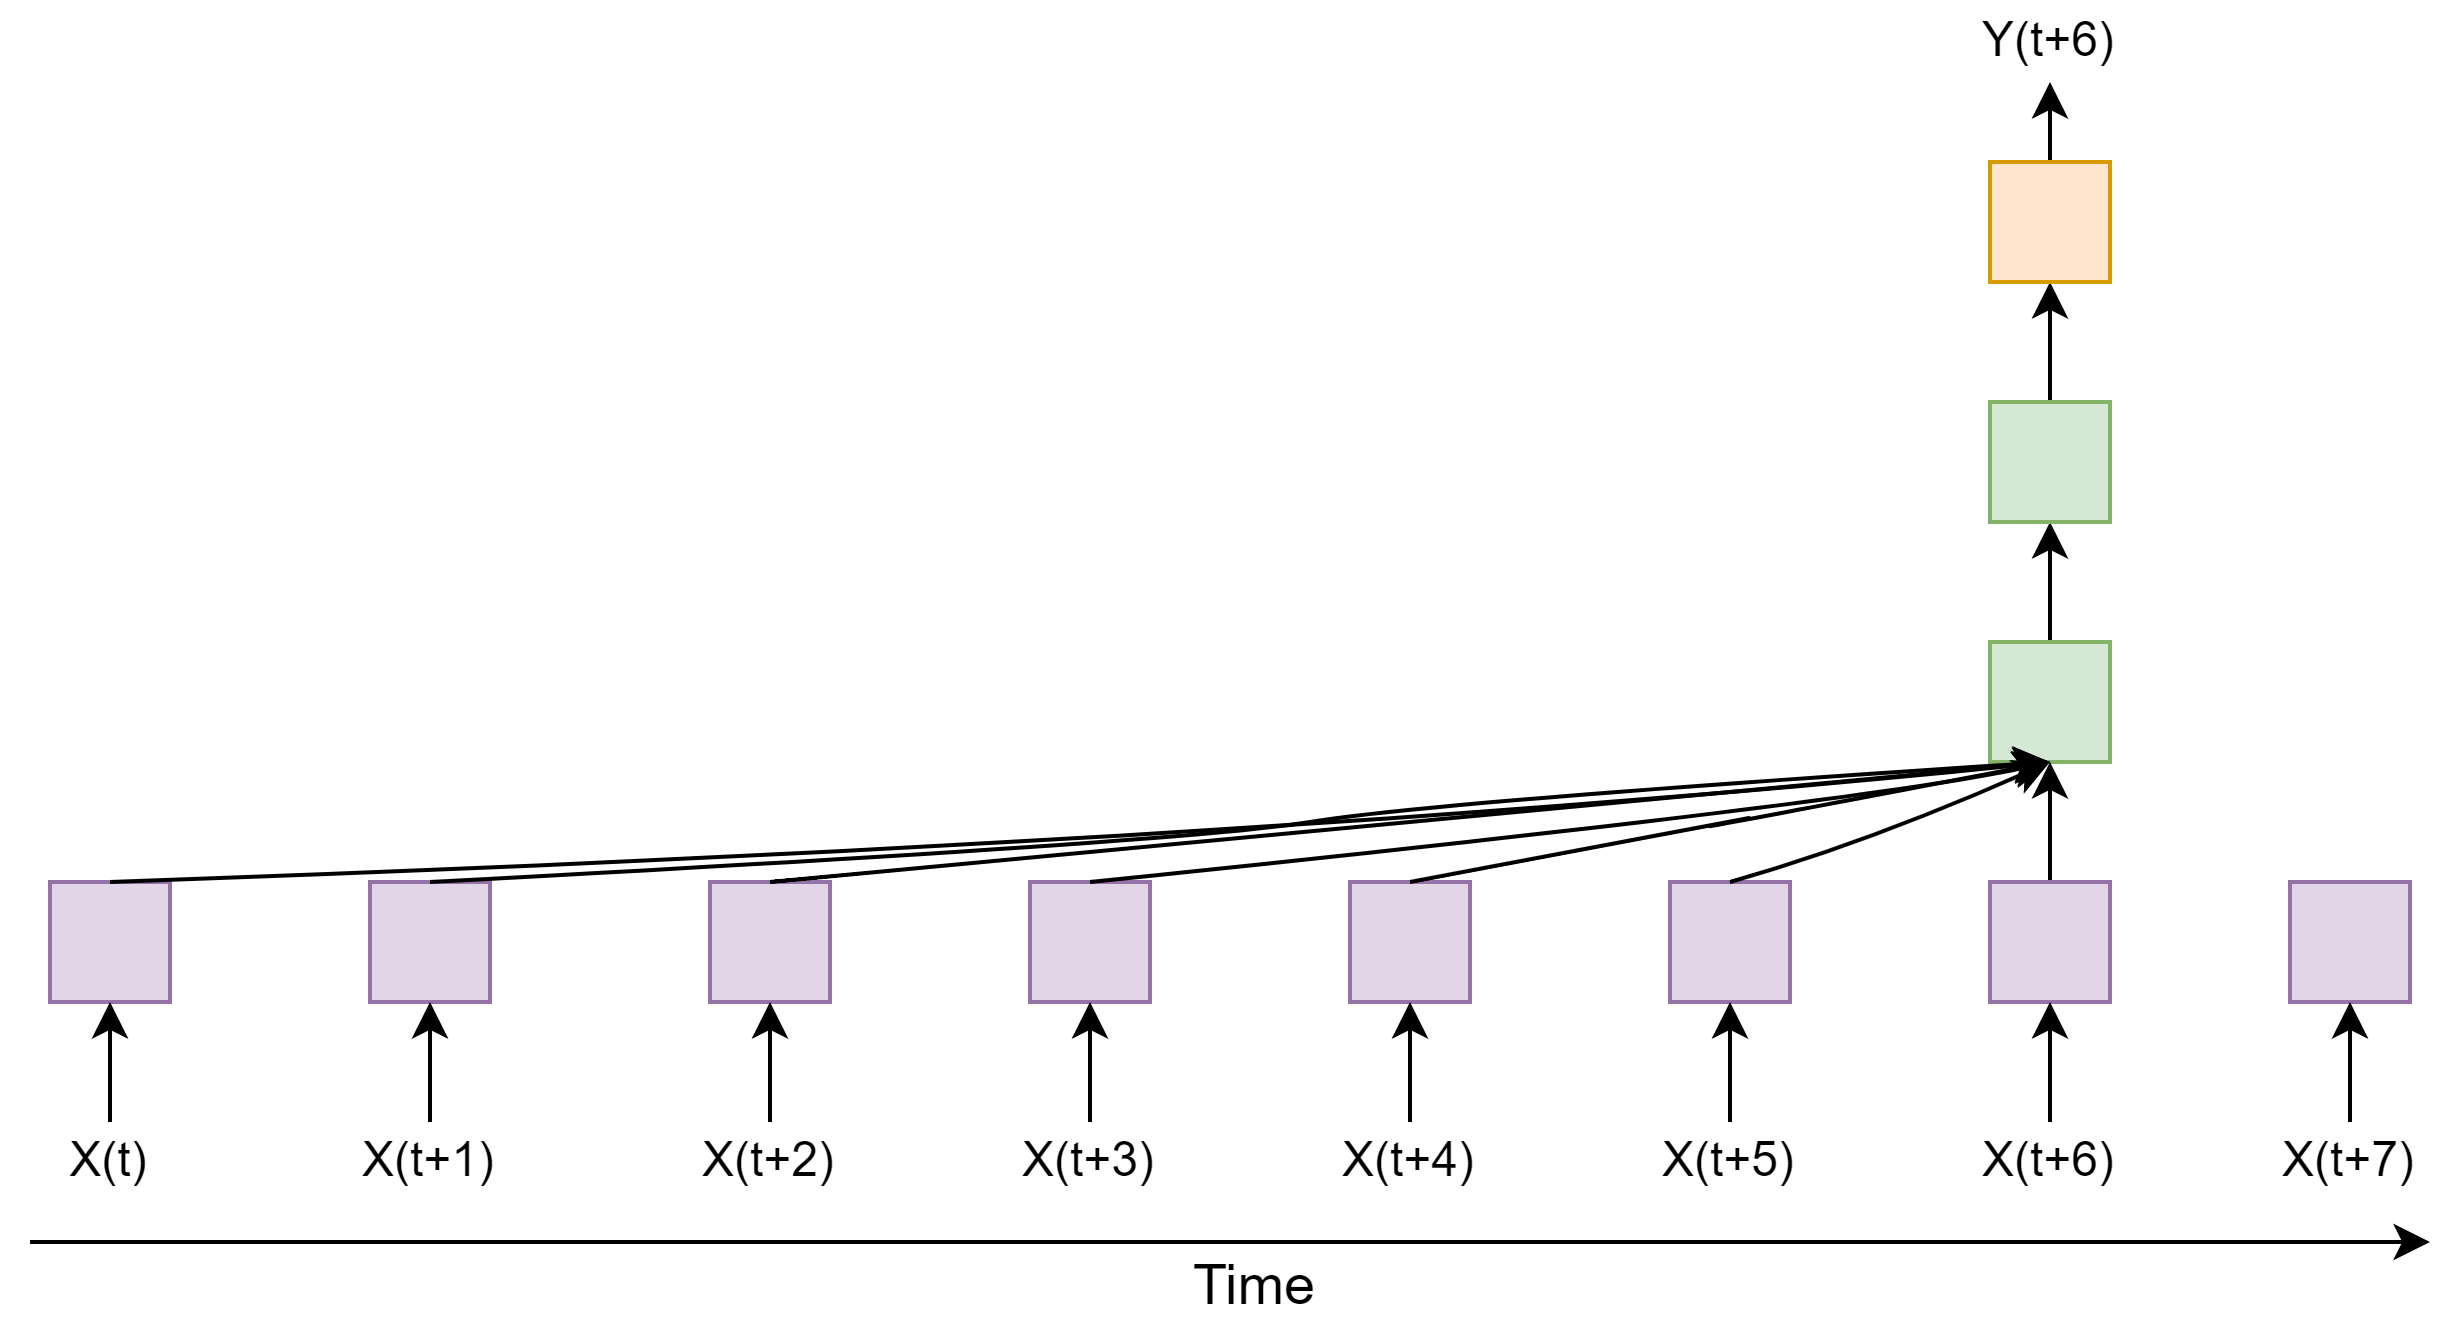
\includegraphics[width=11.2cm, height=6cm]{images/market_network5.png}
    \label{fig:fig7}
\end{figure}
\begin{itemize}
\item Problem: Increasing the “history” makes the
network more complex
\end{itemize}
}

\frame{\frametitle{Long-Term Dependencies}
\begin{figure}
	\centering
    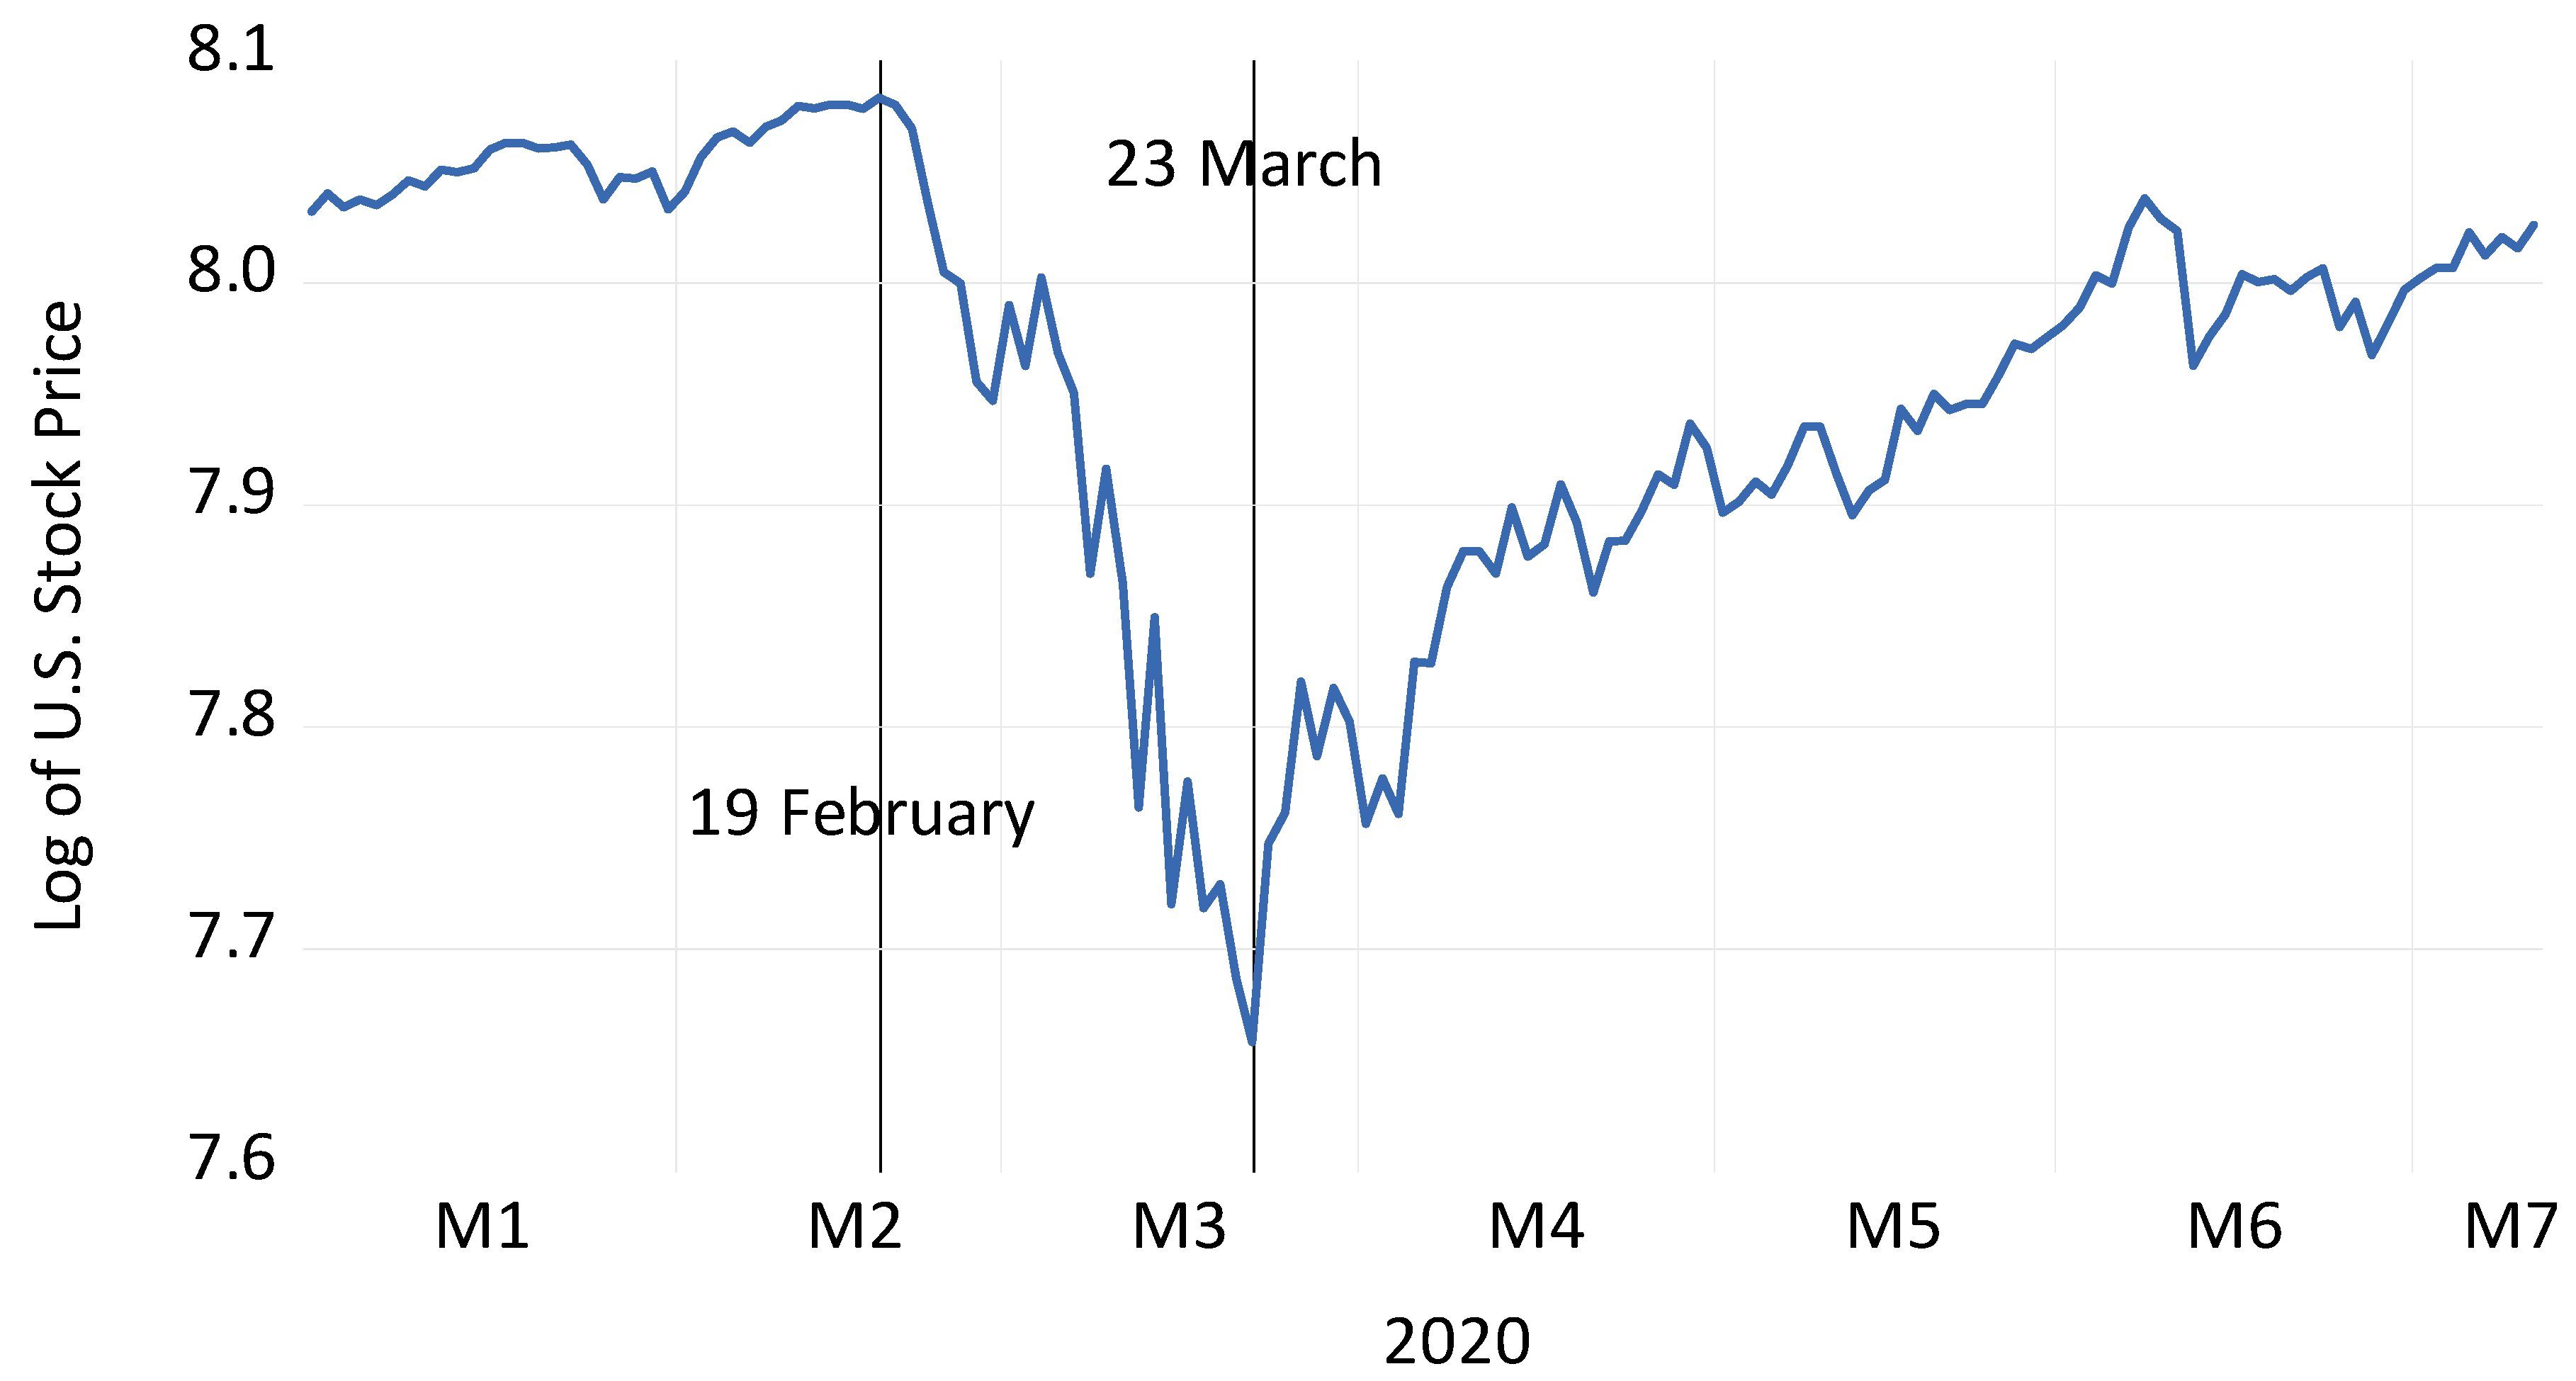
\includegraphics[width=8.5cm]{images/covid19.jpg}
    \label{fig:fig7}
    \caption{The Impact of the COVID-19 Pandemic on the U.S. Economy, \href{https://www.mdpi.com/1911-8074/13/10/233/htm}{source}}
\end{figure}
\vspace{-4mm}
\begin{itemize}
\item Systems often have long-term dependencies
    \begin{itemize}
        \item Weekly/Monthly/Annual trends in the market
        \item Though longer historic events tends to affect us less than more recent events
    \end{itemize}
\item Can you think of an example?
\end{itemize}
}


\frame{\frametitle{Infinite Memory}
\vspace{-5mm}
\begin{figure}
	\centering
    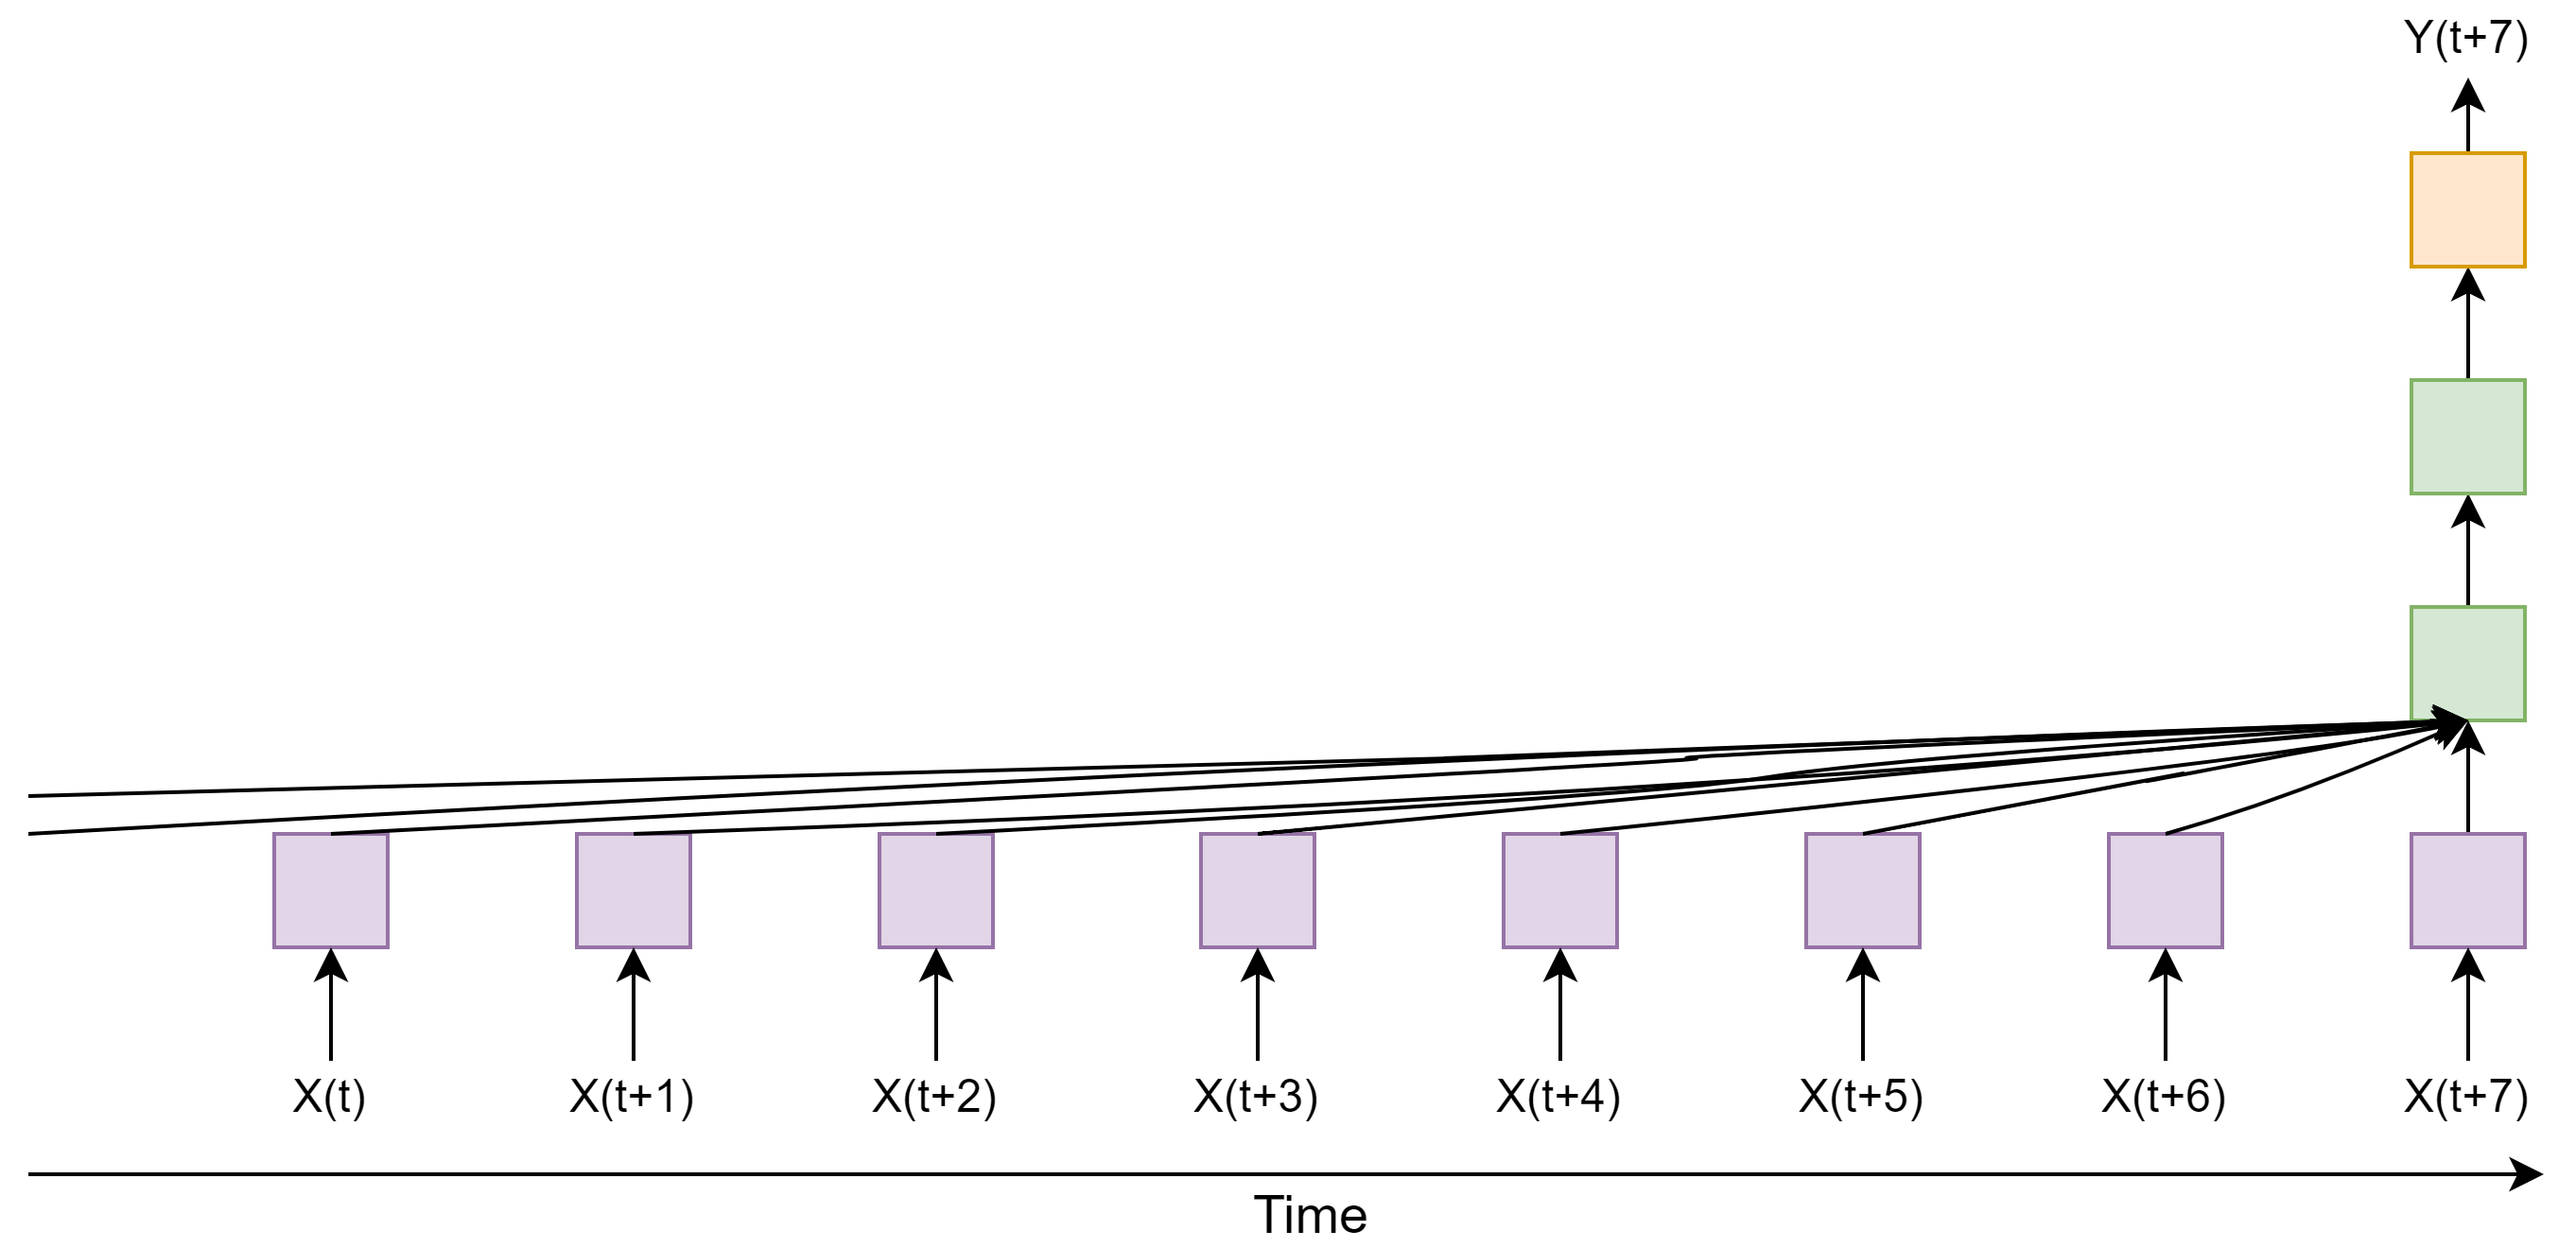
\includegraphics[width=11.2cm, height=6cm]{images/market_network6.png}
    \label{fig:fig7}
\end{figure}
\vspace{-4mm}
\begin{itemize}
\item Infinite response systems
    \begin{itemize}
    \item What happens today can continue to affect the output forever
    \begin{itemize}
        \item Possibly with weaker and weaker influence
    \end{itemize}
    \item $Y_t = f(X_t, X_{t-1},...,X_{t-\infty })$
    \end{itemize}
\end{itemize}
}

\frame{\frametitle{RNN, An Infinite Response System}
\begin{itemize}
    \item We can process a sequence of vectors $x$ by applying a recurrence formula at every time step
    \begin{itemize}
        \item $h_t=f(x_t, h_{t-1}),$ \hspace{4mm} $y_t=g(h_t)$
        \vspace{2mm}
        \item $h_t$ is the state of the network
        \vspace{2mm}
        \item $x_t$ is the input vector at $t$
        \vspace{2mm}
        \item $y_t$ is the output at $t$
        \vspace{2mm}
        \item Need to define initial state $h_{-1}$  for $t=0$
        \vspace{2mm}
        \item An input $x_0$ at $t=0$ produces $h_0$
        \vspace{2mm}
        \item $h_0$ produces $h_1$ which produces $h_2$ and so on...
        \vspace{2mm}
        \item $h_t$ can be produced from $h_{t-1}$ even if $x_t$ is $0$ 
        \vspace{2mm}
        \item A single input influences the output for the rest of time
    \end{itemize}
    \vspace{2mm}
    \item This is a fully recurrent neural network, or simply a recurrent neural network
    \item Don't worry, we will get back to this slide
\end{itemize}
}

\section{Process Sequences}


\frame{\frametitle{Vanilla Neural Networks}
\begin{figure}
	\centering
    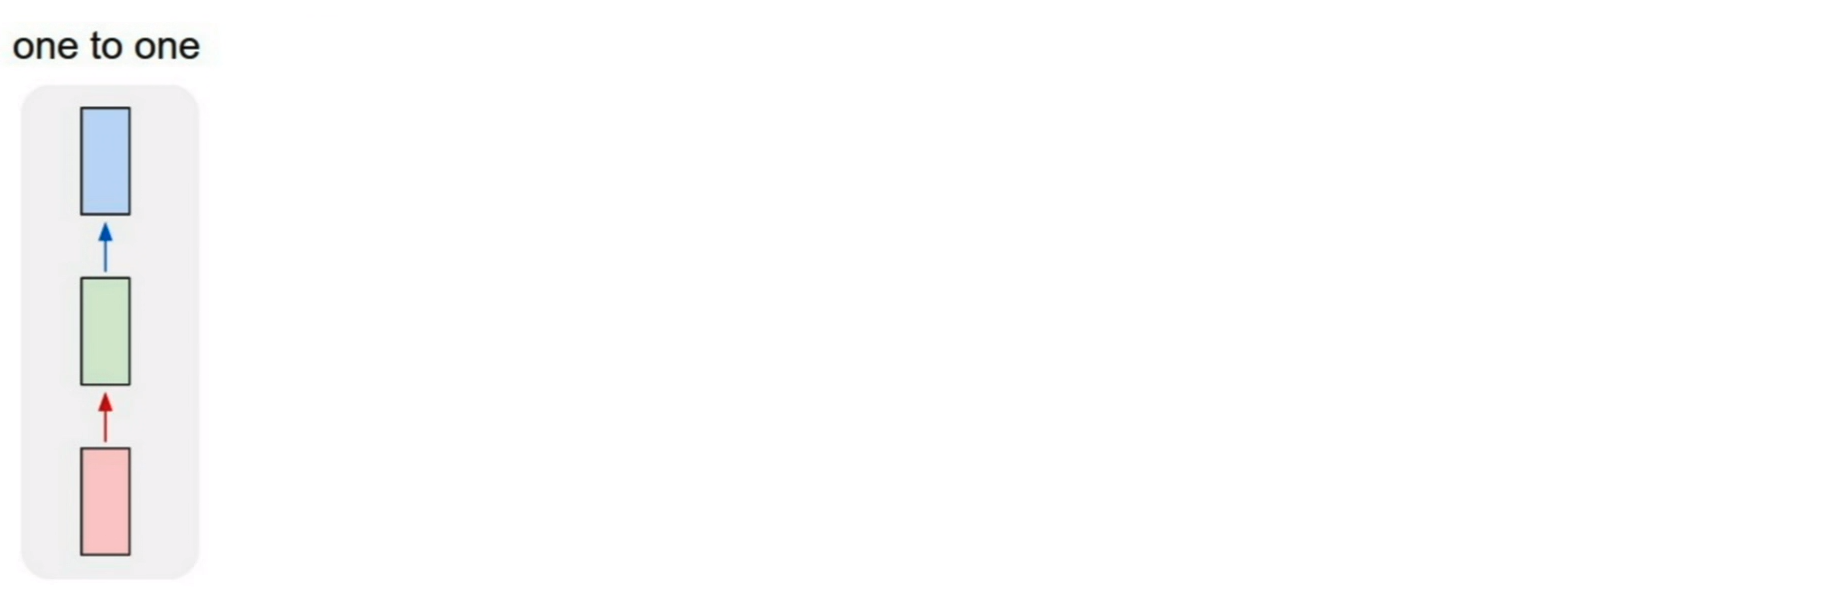
\includegraphics[width=12cm]{images/s1.png}
    \label{fig:fig7}
    \caption{Types of Sequence Problems, \href{https://calvinfeng.gitbook.io/machine-learning-notebook/supervised-learning/recurrent-neural-network/recurrent_neural_networks}{source}}
\end{figure}
\vspace{-4mm}
\begin{itemize}
\item Vanilla Neural Networks
\item Example: Image Classification
\item Fixed-sized input and output
\end{itemize}
}

\frame{\frametitle{Sequence Output}
\begin{figure}
	\centering
    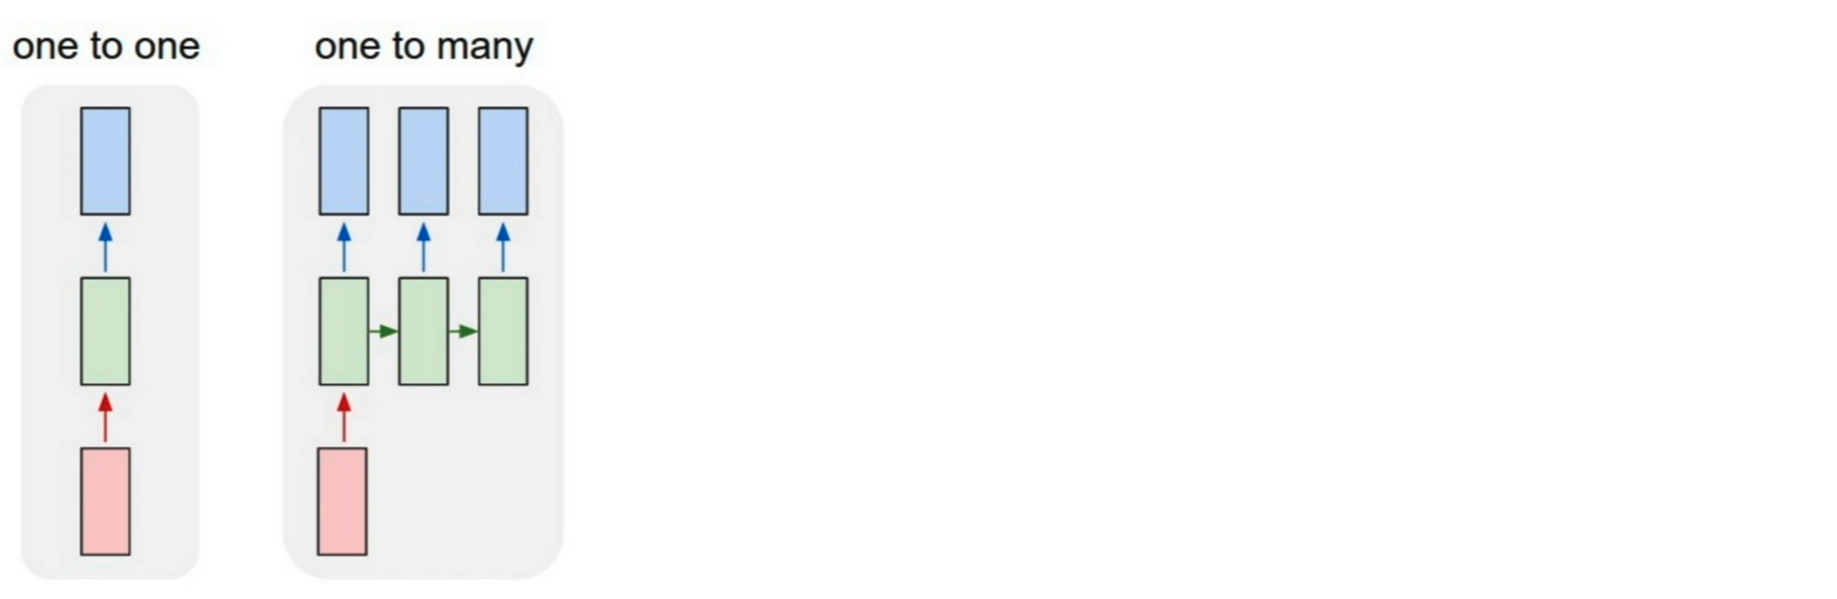
\includegraphics[width=12cm]{images/s2.png}
    \label{fig:fig7}
    \caption{Types of Sequence Problems, \href{https://calvinfeng.gitbook.io/machine-learning-notebook/supervised-learning/recurrent-neural-network/recurrent_neural_networks}{source}}
\end{figure}
\vspace{-4mm}
\begin{itemize}
\item Sequence Output
\item Example: Image Captioning
\item image \rightarrow \hspace{1mm}sequence of words
\end{itemize}
}

\frame{\frametitle{Sequence Input}
\begin{figure}
	\centering
    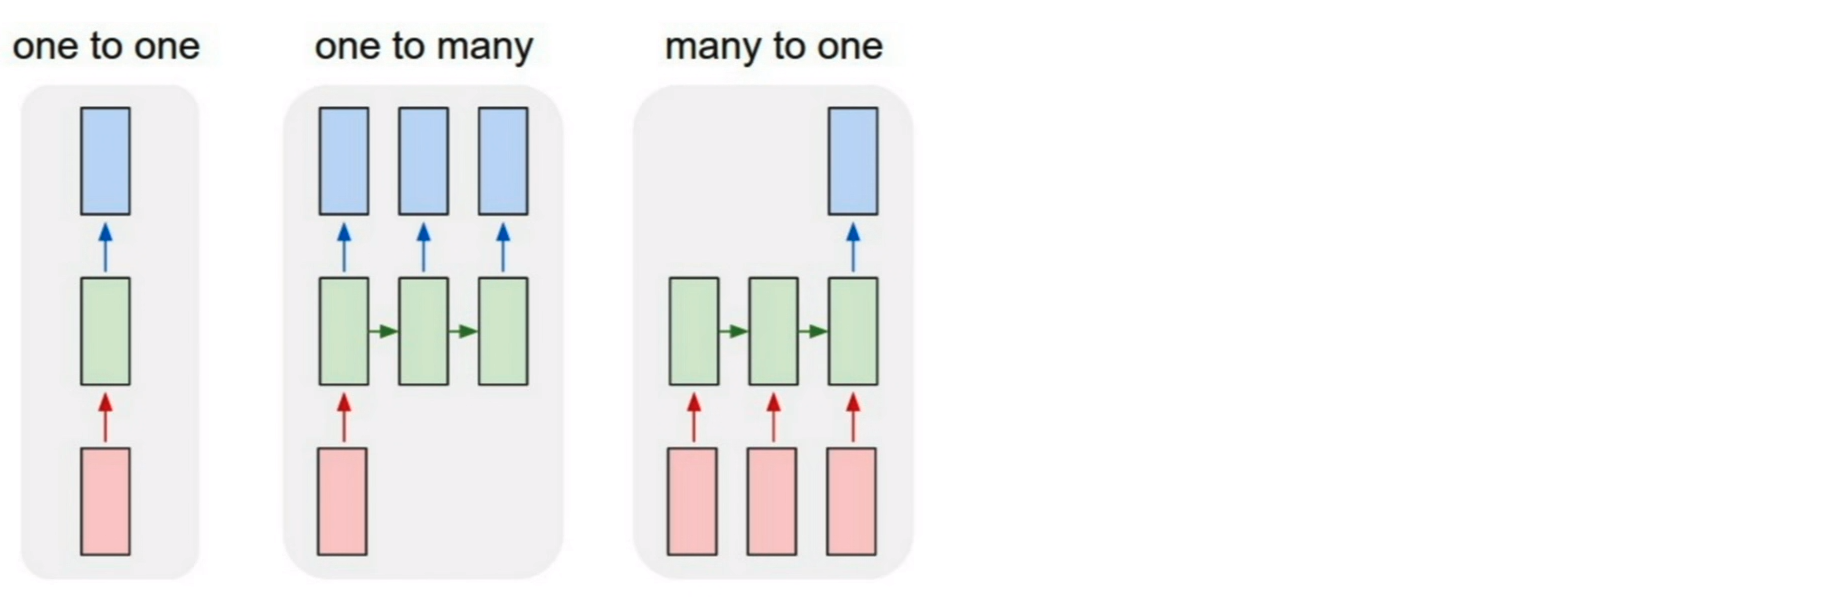
\includegraphics[width=12cm]{images/s3.png}
    \label{fig:fig7}
    \caption{Types of Sequence Problems, \href{https://calvinfeng.gitbook.io/machine-learning-notebook/supervised-learning/recurrent-neural-network/recurrent_neural_networks}{source}}
\end{figure}
\vspace{-4mm}
\begin{itemize}
\item Sequence Input
\item Example: Sentiment Analysis
\item sequence of words \rightarrow \hspace{1mm}sentiment
\end{itemize}
}

\frame{\frametitle{Sequence Input And Sequence Output}
\begin{figure}
	\centering
    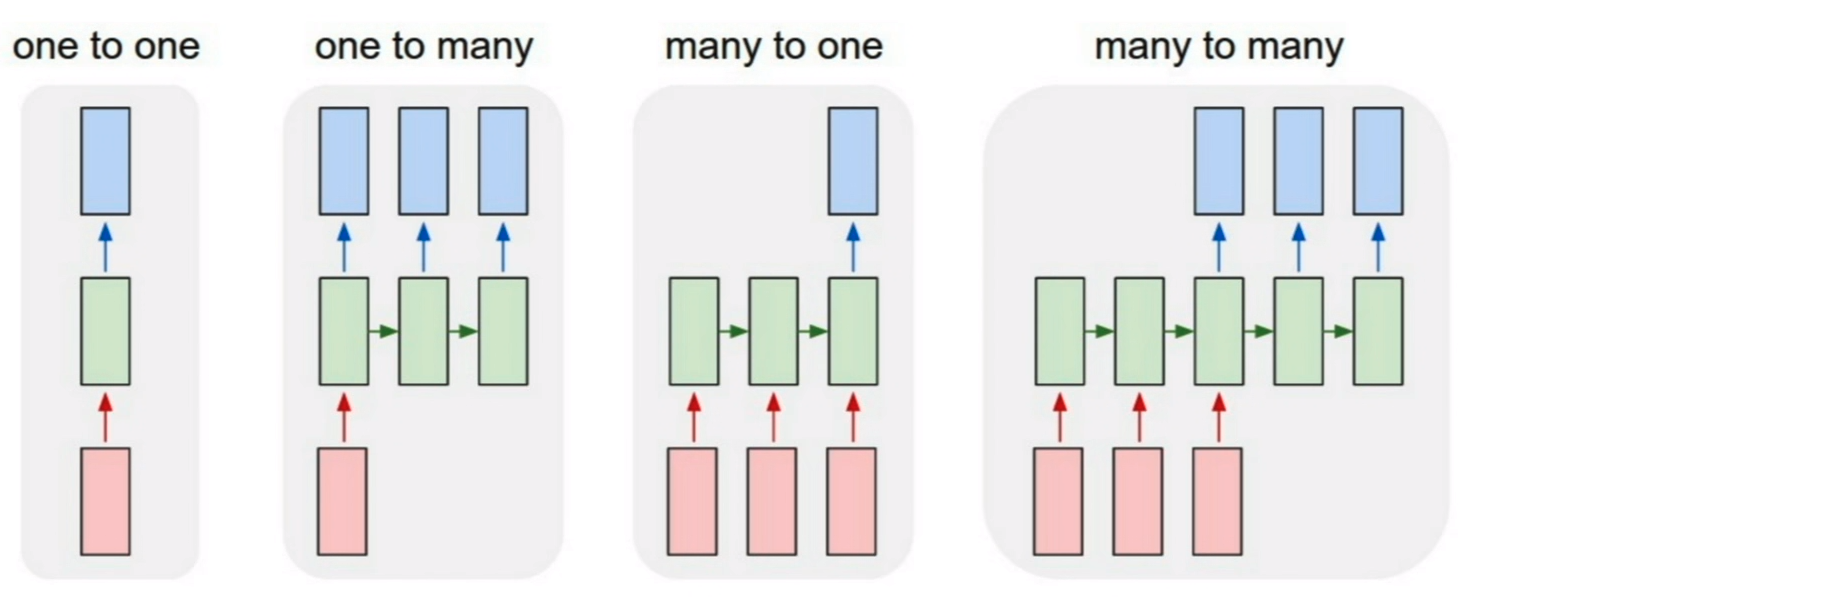
\includegraphics[width=12cm]{images/s4.png}
    \label{fig:fig7}
    \caption{Types of Sequence Problems, \href{https://calvinfeng.gitbook.io/machine-learning-notebook/supervised-learning/recurrent-neural-network/recurrent_neural_networks}{source}}
\end{figure}
\vspace{-4mm}
\begin{itemize}
\item Sequence Input And Sequence Output
\item Example: Machine Translation
\item sequence of words in English \rightarrow \hspace{1mm}sequence of words in Persian
\end{itemize}
}

\frame{\frametitle{Synced Sequence Input And Output}
\begin{figure}
	\centering
    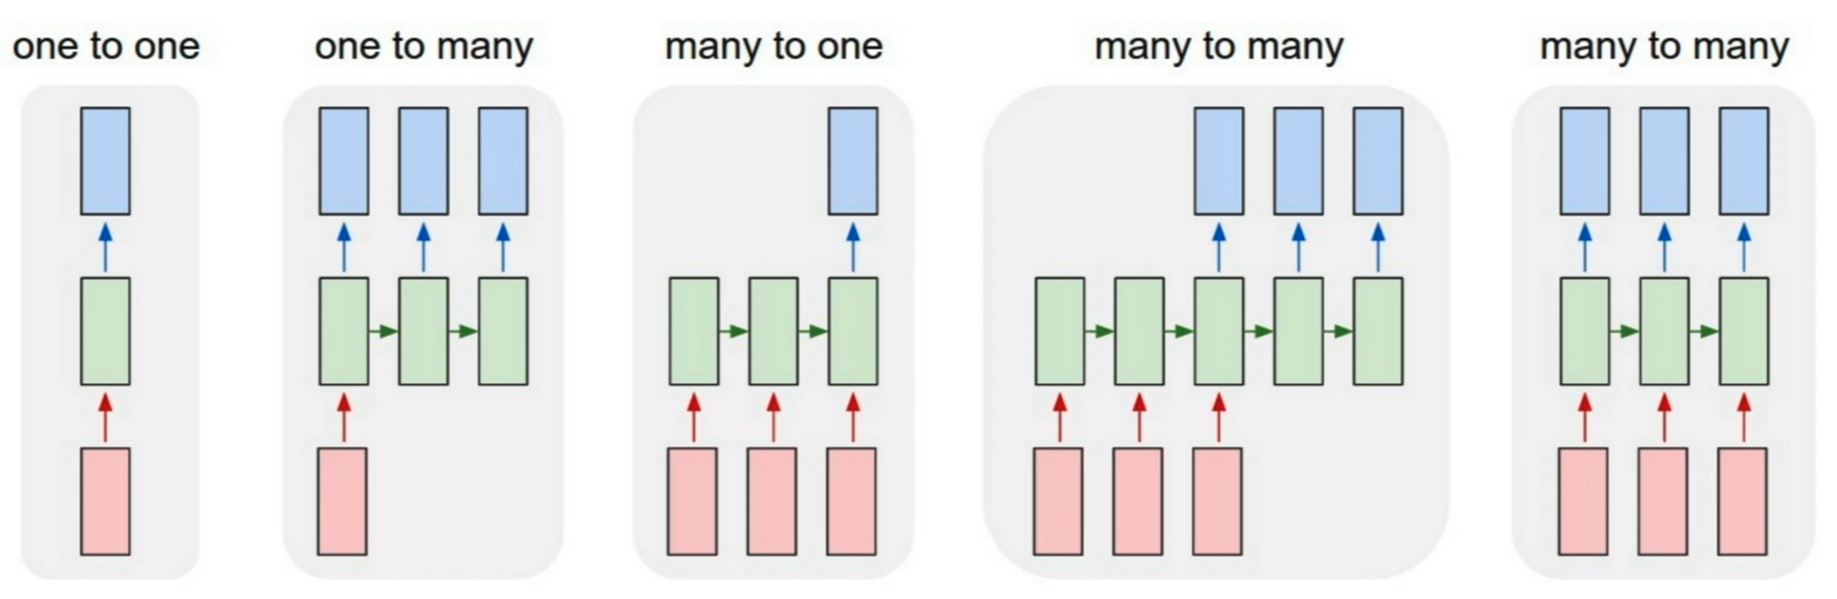
\includegraphics[width=12cm]{images/types2.png}
    \label{fig:fig7}
    \caption{Types of Sequence Problems, \href{https://calvinfeng.gitbook.io/machine-learning-notebook/supervised-learning/recurrent-neural-network/recurrent_neural_networks}{source}}
\end{figure}
\vspace{-4mm}
\begin{itemize}
\item Synced Sequence Input And Output
\item Example: Video Classification
\item frames of the video \rightarrow \hspace{1mm} label of each frame
\end{itemize}
}
\section{RNN}

\frame{\frametitle{Latent Variable Model}
\begin{itemize}
    \item In n-grams for language modeling the conditional probability of token $x_t$  at time step $t$ only depends on the $n$ previous tokens.
    \item If we want to incorporate the possible effect of tokens earlier than time step $t-n$ on $x_t$, we need to increase $n$
    \item By increasing $n$ the number of model parameters would also increase exponentially with it
    \item Hence, rather than modeling $\mathbb{P}(x_t|x_{t-1},...,x_{t-n})$ it is preferable to use a latent variable model:
\end{itemize}
\begin{equation*}
	\centering
    \Large \mathbb{P}(x_t|x_{t-1},...,x_1)\approx \mathbb{P}(x_t|h_{t-1})
\end{equation*}
\begin{itemize}
\item $h_{t-1}$ is a hidden state that stores the sequence information up to time step $t-1$
\item In general, the hidden state at any time step $t$ could be computed based on both the current input $x_t$ and the previous hidden state $h_{t-1}$ :
\begin{equation*}
	\centering
    \Large h_t=f(x_t,h_{t-1})
\end{equation*}
\end{itemize}
}

\frame{\frametitle{Recurrent Neural Network}
\begin{figure}
	\centering
    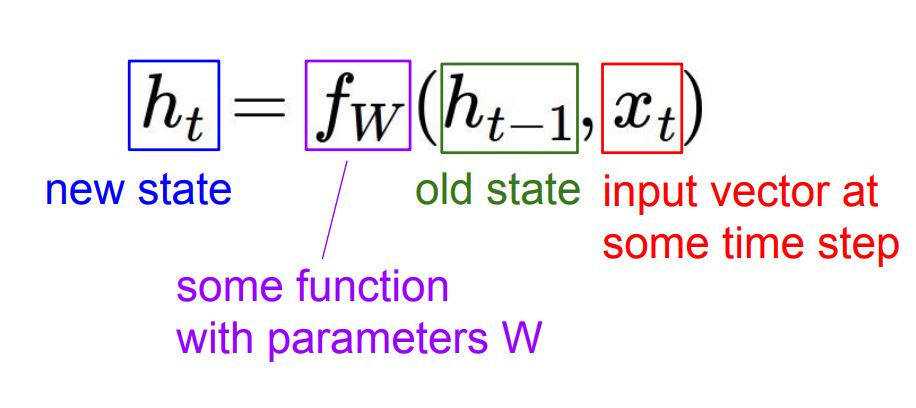
\includegraphics[width=10cm]{images/formula.JPG}
    \label{fig:fig7}
    \caption{RNN formula, \href{http://cs231n.stanford.edu/}{source}}
\end{figure}
\vspace{-4mm}
\begin{itemize}
\item We can process a sequence of vectors x by
applying a recurrence formula at every time step
\item The same function and the same set
of parameters are used at every time step.
\end{itemize}
}

\frame{\frametitle{Vanilla RNN}
\begin{tabular}{lll}
\raisebox{-.5\height}{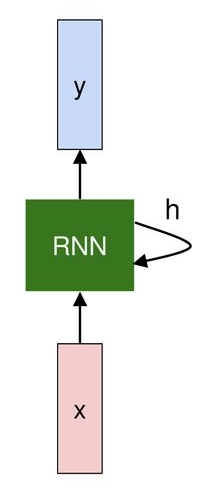
\includegraphics[scale=1]{images/vanilla.png}} & \Large $\begin{matrix}
h_t=f_W(h_{t-1}, x_t)\\ 
y_t=g_W(h_t)\\ \\
\rightarrow \left\{\begin{matrix}
h_t=\tanh(W_{hh}h_{t-1} + W_{hx}x_t + b_h)\\
y_t=W_{yh}h_t+b_y
\end{matrix}\right.
\end{matrix}$
\end{tabular}
}

\frame{\frametitle{RNN: Forward Pass}
\vspace{-4mm}
\begin{figure}
	\centering
    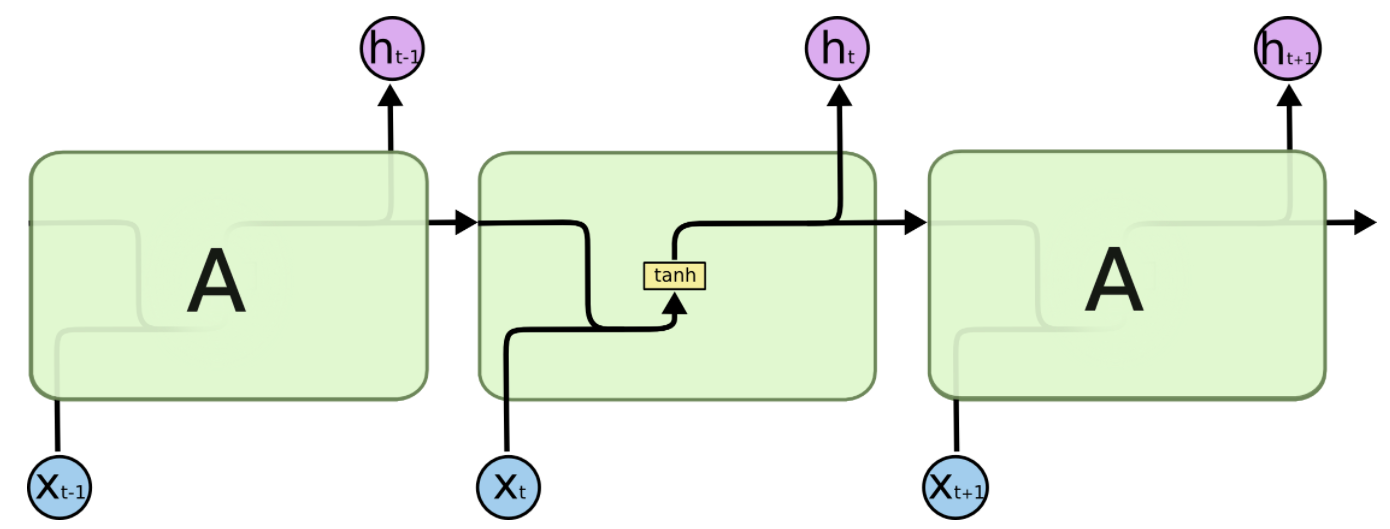
\includegraphics[width=9cm]{images/forward.png}
    \label{fig:fig7}
    \caption{The repeating module in a standard RNN contains a single layer, \href{http://ethen8181.github.io/machine-learning/deep_learning/rnn/2_tensorflow_lstm.html}{source}}
\end{figure}
\centering \large
$h_t=\tanh(W_{hh}h_{t-1} + W_{hx}x_t + b_h)$\\
$=\tanh(\left ( W_{hh} W_{hx} \right ) \begin{pmatrix}
h_{t-1}\\ 
x_t
\end{pmatrix} + b_h)$\\
$=\tanh(W \begin{pmatrix}
h_{t-1}\\ 
x_t
\end{pmatrix} + b_h)$
}

\frame{\frametitle{RNN: Computational Graph}
\begin{figure}
	\centering
    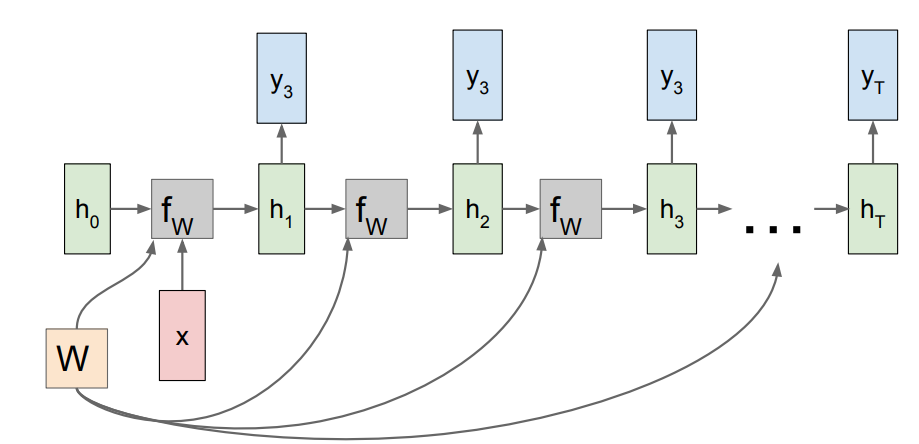
\includegraphics[width=10cm]{images/1m.png}
    \label{fig:fig7}
    \caption{RNN One to Many Computational Graph, \href{https://calvinfeng.gitbook.io/machine-learning-notebook/supervised-learning/recurrent-neural-network/recurrent_neural_networks}{source}}
\end{figure}
}

\frame{\frametitle{RNN: Computational Graph}
\begin{figure}
	\centering
    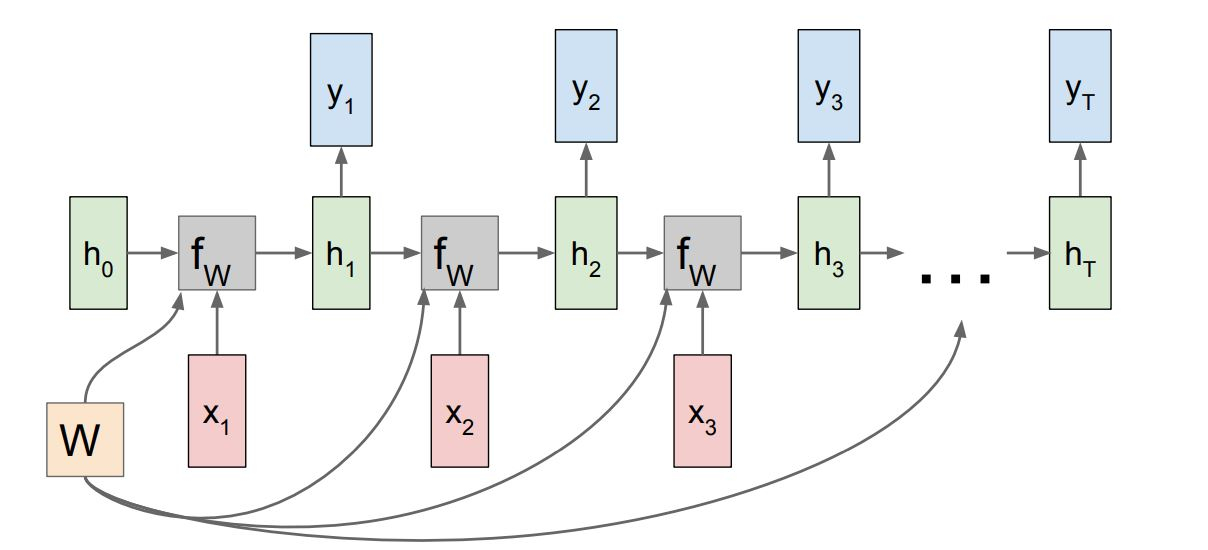
\includegraphics[width=10cm]{images/cgmm.JPG}
    \label{fig:fig7}
    \caption{RNN Many to Many Computational Graph, \href{https://calvinfeng.gitbook.io/machine-learning-notebook/supervised-learning/recurrent-neural-network/recurrent_neural_networks}{source}}
\end{figure}
}

\frame{\frametitle{Example: Character-Level Language Model}
\begin{figure}
	\centering
    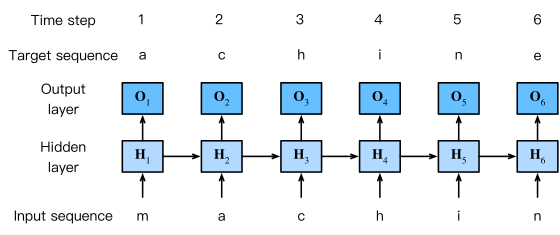
\includegraphics[width=12cm]{images/lm.png}
    \label{fig:fig7}
    \caption{A character-level language model based on the RNN. The input and target sequences are “machin” and “achine”, respectively, \href{https://d2l.ai/chapter_recurrent-neural-networks/rnn.html}{source}}
\end{figure}
}

\frame{\frametitle{Training RNN: Backpropagation Through Time}
\begin{figure}
	\centering
    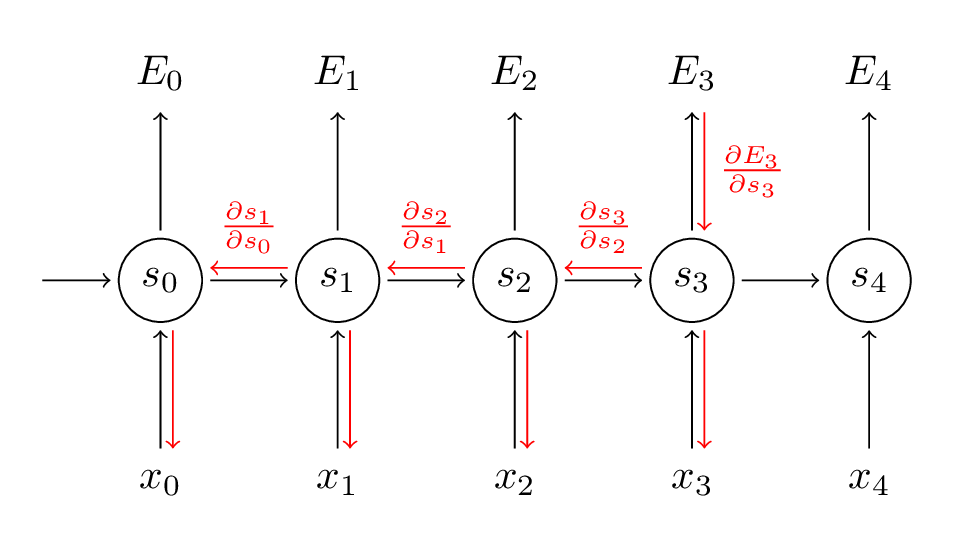
\includegraphics[width=9cm]{images/bptt.png}
    \label{fig:fig7}
\end{figure}
\begin{itemize}
\item We will explain BPTT fully in the next session
\end{itemize}
}

\section{Discussion}
\frame{\frametitle{MLPs vs RNN: The Addition Problem}
\begin{figure}
	\centering
    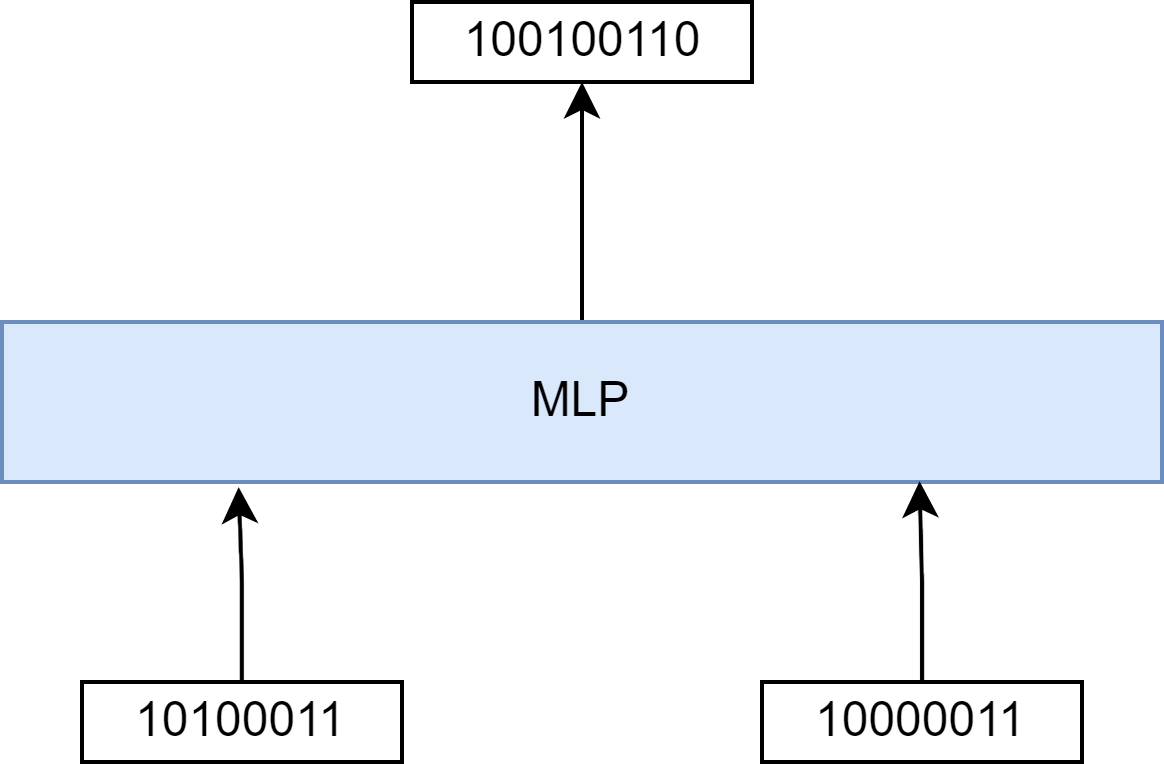
\includegraphics[width=7cm]{images/mlpaddition.png}
    \label{fig:fig7}
\end{figure}
\vspace{-4mm}
\begin{itemize}
\item The addition problem: Add two N-bit numbers to produce a N+1-bit number
\begin{itemize}
    \item Input is binary
    \item MLP will require large number of training instances
    \item Network trained for N-bit numbers will not work for N+1 bit numbers
\end{itemize}
\end{itemize}
}

\frame{\frametitle{MLPs vs RNN: The Addition Problem}
\begin{figure}
	\centering
    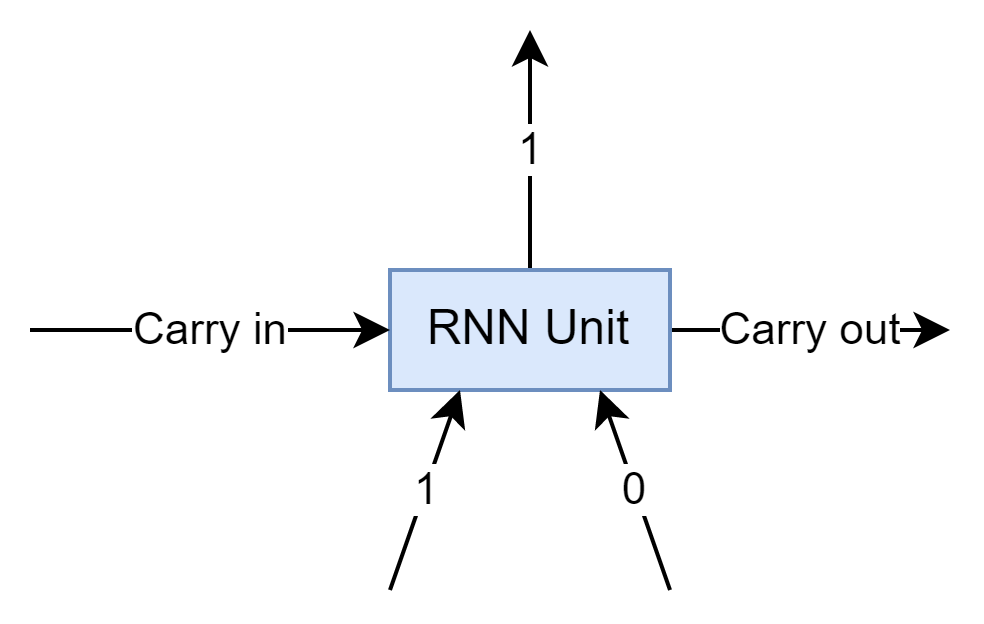
\includegraphics[width=7cm]{images/rnnaddition.png}
    \label{fig:fig7}
\end{figure}
\vspace{-4mm}
\begin{itemize}
\item The addition problem: Add two N-bit numbers to produce a N+1-bit number
\begin{itemize}
    \item RNN solution: Very simple
    \item Can add two numbers of any size
    \item Needs very little training data
\end{itemize}
\end{itemize}
}

\frame{\frametitle{MLPs vs RNN: The Parity Problem}
\begin{figure}
	\centering
    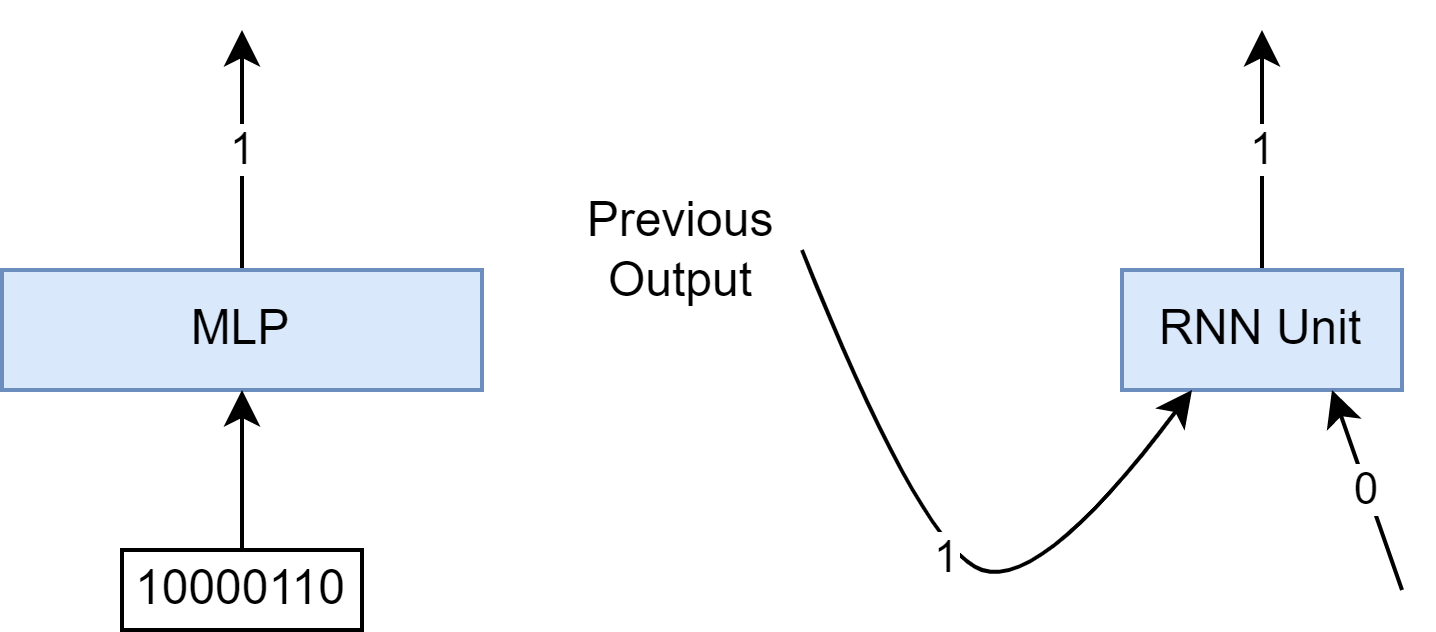
\includegraphics[width=8cm]{images/parity.png}
    \label{fig:fig7}
\end{figure}
\begin{itemize}
\item Is the number of “ones” even or odd
\begin{itemize}
    \item MLP solution: XOR network, quite complex
    \item RNN solution: Simple, generalizes to input of any size
\end{itemize}
\end{itemize}
}

%%%%%%%%%%%%%%%%%%%%%%%%%%%%%%%%%%%%%%%%%%%%%%%%%%%%%%%%%%%%%%%%%%%%%%%%%%%%%%%%%%%%%%%%%%%%%%%
















\frametitle{Final Notes}
\centering
\vspace{50 pt}
\textbf{Thank You!}
\vspace{50pt}

\textbf{Any Question?}
%%%%%%%%%%%%%%%%%%%%%%%%%%%%%%%%%%%%%%%%%%
\end{document}